\documentclass[12pt,oneside,a4paper,parskip]{scrbook}
\usepackage[utf8]{inputenc}
\usepackage{csquotes}
\usepackage[ngerman]{babel}
\usepackage{floatflt}
\usepackage{subfigure}
\usepackage[pdftex]{graphicx}
\usepackage[hidelinks]{hyperref}
\usepackage{color}
\usepackage{amssymb}
\usepackage{textcomp}
\usepackage{nicefrac}
\usepackage{scrhack}
\usepackage{pdfpages}
\usepackage{float}
\usepackage{pdflscape}
\usepackage{subfigure}
\usepackage{pdfpages}
\usepackage[verbose]{placeins}
\usepackage[nouppercase,headsepline,plainfootsepline]{scrpage2}
\usepackage{listings}
\usepackage{xcolor}
\usepackage{color}
\usepackage{caption}
\usepackage{subfigure}
\usepackage{epstopdf}
\usepackage{longtable}
\usepackage{setspace}
\usepackage{booktabs}
\usepackage{hyperref}
\usepackage{enumitem}
\usepackage[style=numeric,backend=bibtex]{biblatex}
\bibliography{literatur}


%%%%%%%%%%%%%%%%%%%
%% definitions
%%%%%%%%%%%%%%%%%%%
\def\BaAuthor{René Ziegler}
\def\BaTitle{Über die Automatisierung der Entwicklung von Software Generatoren}
\def\BaSupervisorOne{Prof.\ Dr.\ Peter Braun}
\def\BaSupervisorTwo{M.Sc. Tobias Fertig}
\def\BaDeadline{\today}

\hypersetup{
pdfauthor={\BaAuthor},
pdftitle={\BaTitle},
pdfsubject={Subject},
pdfkeywords={Keywords}
}

%%%%%%%%%%%%%%%%%%%
%% configs to include
%%%%%%%%%%%%%%%%%%%
\colorlet{punct}{red!60!black}
\definecolor{background}{HTML}{EEEEEE}
\definecolor{delim}{RGB}{20,105,176}
\colorlet{numb}{magenta!60!black}

\definecolor{gray}{rgb}{0.4,0.4,0.4}
\definecolor{darkblue}{rgb}{0.0,0.0,0.6}
\definecolor{cyan}{rgb}{0.0,0.6,0.6}

\definecolor{pblue}{rgb}{0.13,0.13,1}
\definecolor{pgreen}{rgb}{0,0.5,0}
\definecolor{pred}{rgb}{0.9,0,0}
\definecolor{pgrey}{rgb}{0.46,0.45,0.48}

\lstset{
  basicstyle=\ttfamily,
  columns=fullflexible,
  showstringspaces=false,
  commentstyle=\color{gray}\upshape
  linewidth=\textwidth
}

\lstdefinelanguage{json}{
    basicstyle=\normalfont\ttfamily,
    numbers=left,
    numberstyle=\scriptsize,
    stepnumber=1,
    numbersep=8pt,
    showstringspaces=false,
    breaklines=true,
    backgroundcolor=\color{background},
    literate=
     *{0}{{{\color{numb}0}}}{1}
      {1}{{{\color{numb}1}}}{1}
      {2}{{{\color{numb}2}}}{1}
      {3}{{{\color{numb}3}}}{1}
      {4}{{{\color{numb}4}}}{1}
      {5}{{{\color{numb}5}}}{1}
      {6}{{{\color{numb}6}}}{1}
      {7}{{{\color{numb}7}}}{1}
      {8}{{{\color{numb}8}}}{1}
      {9}{{{\color{numb}9}}}{1}
      {:}{{{\color{punct}{:}}}}{1}
      {,}{{{\color{punct}{,}}}}{1}
      {\{}{{{\color{delim}{\{}}}}{1}
      {\}}{{{\color{delim}{\}}}}}{1}
      {[}{{{\color{delim}{[}}}}{1}
      {]}{{{\color{delim}{]}}}}{1},
}

\lstset{language=xml,
  morestring=[b]",
  morestring=[s]{>}{<},
  morecomment=[s]{<?}{?>},
  stringstyle=\color{black},
  numbers=left,
  numberstyle=\scriptsize,
  stepnumber=1,
  numbersep=8pt,
  identifierstyle=\color{darkblue},
  keywordstyle=\color{cyan},
  backgroundcolor=\color{background},
  morekeywords={xmlns,version,type}% list your attributes here
}

\lstset{language=Java,
  showspaces=false,
  showtabs=false,
  tabsize=4,
  breaklines=true,
  keepspaces=true,
  numbers=left,
  numberstyle=\scriptsize,
  stepnumber=1,
  numbersep=8pt,
  showstringspaces=false,
  breakatwhitespace=true,
  commentstyle=\color{pgreen},
  keywordstyle=\color{pblue},
  stringstyle=\color{pred},
  basicstyle=\ttfamily,
  backgroundcolor=\color{background},
%  moredelim=[il][\textcolor{pgrey}]{$$},
%  moredelim=[is][\textcolor{pgrey}]{\%\%}{\%\%}
}


%%%%%%%%%%%%%%%%%%%
%% custom config
%%%%%%%%%%%%%%%%%%%
\setcounter{secnumdepth}{3}
\setcounter{tocdepth}{3}
\begin{document}


%%%%%%%%%%%%%%%%%%%
%% Titelseite
%%%%%%%%%%%%%%%%%%%


\frontmatter
\titlehead{%  {\centering Seitenkopf}
  {Hochschule für angewandte Wissenschaften Würzburg-Schweinfurt\\
   Fakultät Informatik und Wirtschaftsinformatik}}
\subject{Bachelorarbeit}
\title{\BaTitle\\[15mm]}
\subtitle{\normalsize{vorgelegt an der Hochschule f\"{u}r angewandte Wissenschaften W\"{u}rzburg-Schweinfurt in der Fakult\"{a}t Informatik und Wirtschaftsinformatik zum Abschluss eines Studiums im Studiengang Informatik}}
\author{\BaAuthor}
\date{\normalsize{Eingereicht am: \BaDeadline}}
\publishers{
  \normalsize{Erstpr\"{u}fer: \BaSupervisorOne}\\
  \normalsize{Zweitpr\"{u}fer: \BaSupervisorTwo}\\
}

%\uppertitleback{ }
%\lowertitleback{ }

\maketitle


%%%%%%%%%%%%%%%%%%%
%% abstract
%%%%%%%%%%%%%%%%%%%

\section*{Zusammenfassung}

TODO

\section*{Abstract}

TODO

\newpage
\chapter*{Danksagung}



%%%%%%%%%%%%%%%%%%%
%% Inhaltsverzeichnis
%%%%%%%%%%%%%%%%%%%
\tableofcontents



%%%%%%%%%%%%%%%%%%%
%% Main part of the thesis
%%%%%%%%%%%%%%%%%%%
\mainmatter


\chapter{Einführung}\label{ch:intro}

Als Henry Ford 1913 die Produktion des Modell T, umgangssprachlich auch Tin Lizzie genannt, auf Fließbandfertigung umstellte, revolutionierte er die Automobilindustrie. Ford war nicht der erste, der diese Form der Automatisierung verwendete. Bereits 1830 kam in den Schlachthöfen von Chicago eine Maschine zum Einsatz, die an Fleischerhaken aufgehängte Tierkörper durch die Schlachterei transportierte. Bei der Produktion des Oldsmobile Curved Dash lies Ranson Eli Olds 1910 erstmals die verschiedenen Arbeitsschritte an unterschiedlichen Arbeitsstationen durchführen. Fords Revolution war die Kombination beider Ideen. Er entwickelte eine Produktionsstraße, auf welcher die Karossen auf einem Fließband von Arbeitsstation zu Arbeitsstation befördert wurden. An jeder Haltestelle wurden nur wenige Handgriffe von spezialisierten Arbeitern durchgeführt\,\cite{sagerso2008}.

Fords Vision war es, ein Auto herzustellen, welches sich Menschen aller Gesellschaftsschichten leisten konnten. Durch die Reduktion der Produktionszeit der Tin Lizzie von 12,5 Stunden auf etwa 6 Stunden konnte Ford den Preis senken. Kostete ein Auto des Model T vor der Einführung der Produktionsstraße 825\$, erreichte der Preis in den Jahren danach einen Tiefststand von 259\$\,\cite{reichlesz2010}. Setzt man diesen Preis in ein Verhältnis mit dem durchschnittlichen Einkommen in den USA, das 1910 bei jährlich 438\$ lag, kann man sagen, dass Fords Traum durch die eingesetzten Techniken Realität wurde\,\cite{usembassyodnumbers}.

Im Zuge der weiteren Entwicklung der Robotik wurden immer mehr Aufgaben, die bisher von Menschen am Fließband durchgeführt wurden, von Automaten übernommen. In der Automobil-Industrie war General Motors der erste Hersteller, bei welchem die Produktionsstraßen im Jahr 1961 mit 66 Robotern des Typs Unimation ausgestattet wurden. Bis zur Erfindung des integrierten Schaltkreises in den 1970ern waren die Roboter ineffizient. Der Markt für industrielle Roboter explodierte jedoch in den Folgejahren. Im Jahr 1984 waren weltweit ungefähr 100.000 Roboter im Einsatz\,\cite{czaeis2000, wallen2008}.

Die industrielle Revolution prägte die Autoindustrie: von der Erfindung auswechselbarer Teile 1910 bei Ransom Olds, über die Weiterentwicklung des Konzepts unter der Verwendung von Fließbändern bei Ford im Jahr 1913, bis hin zur abschließenden Automatisierung mit Industriellen Robotern in den frühen 1980ern\,\cite{czaeis2000}.

\section{Motivation}

\begin{quote}
	\glqq If you can compose components manually, you can also automate this process.\grqq
\end{quote}

Das hervorgehobene Zitat nennen Czarnecki und Eisenecker die Automation Assumption. Diese allgemein gehaltene Aussage lässt die Parallelen, die die beiden Autoren zwischen der Automatisierung der Automobilindustrie und der automatischen Code Generierung sehen, erkennen. Dafür müssten die einzelnen Komponenten einer Softwarefamilie derart gestaltet werden, dass diese austauschbar in eine gemeinsame Struktur integriert werden können. Des weiteren müsste klar definiert sein, welche Teile eines Programms konfigurierbar seien und welche der einzelnen Komponenten in welcher Konfiguration benötigt werden. Setzt man dieses definierte Wissen in Programmcode um, könnte ein solches Programm eine Software in einer entsprechenden Konfiguration generieren\,\cite{czaeis2000}.

Konkret bedeutet dies, dass entweder eine vorhandene Implementierung in Komponenten zerlegt werden muss oder eine für die Zwecke der Codegenerierung vorgesehene Referenzimplementierung geschrieben wird. Codeabschnitte, die in Ihrer Struktur gleich sind, sich jedoch inhaltlich unterscheiden, müssen formal beschrieben werden\,\cite{stahl2007}. Ein solches abstraktes Modell wird dann mit Daten befüllt. Schlussendlich wird ein Generator implementiert, der den Quellcode für unterschiedliche Ausprägungen eines Programms einer Software-Familie, auf Basis des konkreten Modells, generieren kann\,\cite{fowler2010}.

Sowohl bei der Umsetzung von einzigartigen Anwendungen, als auch bei der Verwirklichung von Software mit mehreren Varianten, kann die Verwendung von bereits verfügbaren Code Generatoren oder die Entwicklung eigener Code Generatoren vorteilhaft sein. Die Entwicklungsgeschwindigkeit könnte erhöht, die Softwarequalität gesteigert und Komplexität durch Abstraktion reduziert werden\,\cite{stahl2007}. Allgemein wird weniger Zeit benötigt, um eine größere Vielfalt an ähnlichen Programmen zu entwickeln\,\cite{czaeis2000}.

Bisher müssen fast alle Teilaufgaben bei der Umsetzung eines Code Generators manuell durchgeführt werden. Werkzeuge wie Language Workbenches können Code bis zu einem gewissen Grad automatisiert generieren oder interpretieren. Sie haben aber in erster Linie die Aufgabe, den Entwickler beim Design von externen domänenspezifischen Sprachen zu unterstützen und dienen als Entwicklungsumgebung für die Arbeit mit der Sprache\,\cite{fowler2010}.

Soll ein Projekt Modellgetrieben entwickelt werden, so lohnt sich dies wirtschaftlich gesehen erst, wenn auf Basis des entwickelten Modells mehrere Programme entwickelt wurden\,\cite{}. Einer der Teilschritte dieses Entwicklungsprozesses ist die Planung und Implementation des Code Generators. Durch ihre hohe Komplexität, ist diese Aufgabe sehr zeitaufwendig\,\cite{}.

ÜBERARBEITEN
\section{Zielsetzung}

In dieser Arbeit soll untersucht werden, ob und wie die Entwicklung eines Codegenerators automatisiert werden kann. Eine zusätzliche Ebene der Indirektion könnte das komplexe Thema der Modellgetriebenen Softwareentwicklung weiter vereinfachen und somit Codegenerierung auch wirtschaftlicher machen.

Im speziellen wird analysiert, wie ein Metagenerator zur Erhöhung der Wirtschaftlichkeit modellgetriebener Softwareentwicklung umgesetzt werden könnte. Zu diesem Zweck wird eine beispielhafte Java Anwendung erarbeitet, welche es ermöglichen soll, aus vorhandenem Java Quelltext einen Metagenerator zu erzeugen.

Ein Metagenerator bezeichnet hierbei einen Softwaregenerator welcher auf Basis einer Referenzimplementation, vollständig oder in Teilen, die Entwicklung anderer Softwaregeneratoren automatisiert.

\section{Aufbau der Arbeit}

Die sieben Kapitel dieser Bachelorarbeit versuchen den Leser Stück für Stück an das komplexe Thema der Metagenerierung heranzuführen. Da es nicht möglich ist im Rahmen einer vergleichsweise kurzen Thesis wie dieser sämtliche Grundlagen der Informatik zu beschreiben, wird ein solides Fundament aus Vorwissen, wie man es zum Beispiel in einem Bachelorstudium erwerben kann, vorausgesetzt.

Eingeleitet wird diese Arbeit mit einem Kapitel zur Motivation und Zielsetzung, in welchem aufgezeigt werden soll warum es sinnvoll ist, sich mit dem Thema der modellgetriebene Softwareentwicklung zu beschäftigen. 

Das zweite Kapitel behandelt die erweiterten, grundlegenden Kenntnisse, die zum Verständnis des Textes notwendig sind. Hier wird sowohl auf die modellgetriebene Softwareentwicklung, als auch auf die Software Architektur und die Verwendung von Design Pattern objektorientierter Programmierung eingegangen.

Aufbauend auf dem vorhergehenden Abschnitt sollte das dritte Kapitel, die Analyse, gut verständlich sein. Hier wird zuerst der wirtschaftliche Aufwand konventioneller Softwareprojekte mit dem Aufwand von Projekten welche ein modellgetriebenen Ansatz verfolgen verglichen. Danach werden die Probleme der einzelnen Teilschritte bei der Automatisierung der Entwicklung des Codegenerators untersucht.

Das Konzept Kapitel erläutert nun den im Proof-of-Concept verfolgten Lösungsansatz der analysierten Probleme. Zur Veranschaulichung kommen hier lediglich Diagramme zum Einsatz, dadurch sollte es möglich sein die allgemeine Idee hinter der Implementation leichter zu verstehen und den Ansatz losgelöst von der Umsetzung weiter zu verfolgen.

Im fünften Kapitel werden jetzt zum einen die verwendeten externen Bibliotheken kurz vorgestellt, zum anderen wird genau auf die Architektur der entwickelten Anwendung eingegangen. Die Funktionsweise und der Aufbau jeder Programmkomponente wird anhand von Quelltext Auszügen genau erläutert, mithilfe von Beispielen wird die Verwendung der einzelnen Einheiten demonstriert.

Das vorletzte Kapitel der Arbeit evaluiert sowohl das Konzept als auch die Umsetzung aller Module im Detail. Außerdem wird die allgemeine Softwarequalität des entwickelten Generators nach bewährten Kriterien untersucht. Besonders umfangreich werden die Grenzen des Lösungsansatzes diskutiert und mögliche Antworten auf die hieraus entstehenden Fragen angesprochen.

Mit dem siebten Kapitel werden Inhalt und Erkenntnisse der Arbeit noch einmal in gebündelter Form zur Verfügung gestellt. Ein ausführlicher Ausblick soll die vielen möglichen Anknüpfungspunkte dieser Thesis aufzeigen.

\chapter{Grundlagen}

Um die grundlegenden Zusammenhänge zu verstehen wird im folgenden auf die verschiedenen Aspekte und Teilschritte der modellgetriebenen Softwareentwicklung eingegangen. Begriffe und Konzepte die in der Arbeit zur Anwendung kommen, werden eingeführt und definiert. Danach wird auf einige Grundlagen der Softwarearchitektur, vor allem auf die Prinzipien der Softwaretechnik eingegangen. Da in der Implementation auf einige Design Pattern objektorientierter Programmierung zurückgegriffen wird, werden deren Zweck, Aufbau und Anwendbarkeit abschließend in diesem Kapitel erläutert.

\section{Modellgetriebene Softwareentwicklung (MDSD)}

\begin{quote}\glqq Modellgetriebene Softwareentwicklung (Model Driven Software Development, MDSD) ist ein Oberbegriff für Techniken, die aus formalen Modellen automatisiert lauffähige Software erzeugen.\grqq \end{quote}

Die obige Definition stammt aus dem Buch modellgetriebene Softwareentwicklung von Thomas Stahl und Markus Völter\,\cite[S. 11]{stahl2007}. Sie lässt sich gut erläutern wenn man sie in drei Teile zerlegt.

Zunächst einmal wäre dort der Ausdruck "formales Modell". Damit ist ein Modell gemeint welches einen Teil einer Software vollständig beschreibt. Jedoch soll das nicht heißen, dass dieses Modell allumfassend ist, sondern was genau von diesem Modell beschrieben wird muss eindeutig reguliert sein\,\cite[S. 11f.]{stahl2007}. Weiterhin bezieht sich die Definition darauf dass lauffähige Software erzeugt wird. D. h. wird das formale Modell nur zur Dokumentation verwendet oder dient es als Information zur händischen Umsetzung, so kann man das laut Stahl und Völter nicht als modellgetriebene Softwareentwicklung bezeichnen\,\cite[S. 12]{stahl2007}. Der letzte Teil der Definition den die Autoren explizit erläutern ist, dass die Umwandlung von Modell zu ausführbar Software automatisiert erfolgen soll. Insbesondere soll der Quelltext nicht nur einmal generiert und dann manuell verändert und weiterentwickelt werden, sondern das Modell soll anstelle des Quelltextes treten. Der Quelltext wird aus den geänderten Modellen generiert, dadurch kann aktueller und einheitlicher Quellcode gewährleistet werden\,\cite[S. 13]{stahl2007}.

In der Literatur findet sich auch die alternative Bezeichnung Model Driven Development (MDD)\,\cite{selic2003,atkinson2003}. Diese Thesis wird jedoch durchgängig die Bezeichnung MDSD verwenden.

Auch der Model Driven Architecture (MDA) Ansatz der Object Management Group (OMG) beschäftigt sich mit modellgetriebener Softwareentwicklung\,\cite{mdaguide}. Dieser Ansatz beschreibt detailliert und umfassend den Gesamtprozess von der Analyse bis hin zur Implementation und führt eigene Standards ein. 

Czarnecki und Eisenecker verwenden den Ausdruck Generative Programming, definieren ihn jedoch in den wesentlichen Punkten vergleichbar zu MDSD. Wobei Generative Programming nach Czarnecki und Eisenecker nach vollständiger Automation strebt und ein vollständiges Zwischen- oder Endprodukt erzeugen soll\,\cite[S. 5]{czaeis2000}. Für MDSD merken Stahl und Völter an, dass die verwendeten Modelle nicht unbedingt das vollständige System abbilden, ein komplettes System enthalte sowohl manuell implementierte als auch automatisch generierte Anteile\,\cite[S. 13]{stahl2007}.

Durch MDSD soll, wie bereits in der Einleitung dieser Arbeit beschrieben, die Qualität der entstandenen Software gesteigert werden. Dies wird durch den resultierenden einheitlichen Code und die erhöhte Wiederverwertbarkeit erreicht. Außerdem kann potentiell mithilfe der zusätzlichen Abstraktion eine erhöhte Entwicklungsgeschwindigkeit erzielt werden. Ein Bonus von MDSD ist es, dass die Software immer durch aktuelle Modelle beschrieben und somit zumindest in Teilen dokumentiert wird\,\cite[S. 13ff.]{stahl2007}. Die Vorteile von Generative Programming\,\cite[S. 13ff.]{czaeis2000} und MDA\,\cite{mdaguide} werden sehr Ähnlich beschrieben.

\subsection{Domäne}

Bei der modellgetriebenen Softwareentwicklung sind, wie bereits erwähnt, Modelle Dreh und Angelpunkt des Entwicklungsprozesses. Um jedoch ein Modell bilden zu können muss zuerst untersucht werden was mit diesem Modell abgebildet wird. Diese Untersuchung ist Teil des Domain Engineerings.

Domain Engineering umfasst die Analyse das Design und die Implementation einer Domäne. Design und Implementation beziehen sich bereits auf die Zusammensetzung des Systems und dessen technische Umsetzung\,\cite[S. 21f.]{czaeis2000}. Zur Modellbildung ist für diese Arbeit vor allem die Domänenanalyse interesannt.

\subsubsection{Definition}

Eine Domäne beinhaltet laut Czarnecki und Eisenecker das fachliche Wissen über ein Problem-Themengebiet. Jedoch geht die Domäne im Domain Engineering noch darüber hinaus. Sie umfasst nicht nur das fachliche Wissen, sondern auch Informationen darüber wie Anwendungen für diesen Themenbereich aufgebaut sind. Wichtig ist hierbei, dass die Domäne sich aus dem übereinstimmenden Wissen der beteiligten Stakeholder ergibt. Wobei hier alle Personen die ein Interesse an einer bestimmten Domäne haben als Stakeholder bezeichnet werden\,\cite[S. 33]{czaeis2000}.

\subsubsection{Domänenanalyse}

Bereits im 1990 erschienenen Paper Domain Analysis: An Introduction zählt der Autor Rubén Prieto-Díaz die drei Grundschritte zur Analyse einer Domäne auf\,\cite{prieto1990}:

\begin{enumerate}[itemsep=-10pt]
	\item identification of reusable entities 
	\item abstraction or generalization 
	\item classification and cataloging for further reuse
\end{enumerate}

Diese drei Punkte sind auch heute noch zutreffend. In der Analyse wird zunächst beim Domain Scoping die Domäne eingegrenzt. Dies ist notwendig um eine konsistente Umsetzung möglich zu machen und alle Anforderungen konkret und klar zu definieren\,\cite[S. 239]{stahl2007}. Danach werden im allgemeinen Entitäten, Operationen und Beziehungen zwischen diesen identifiziert. Sobald dies geschehen ist, können diese auf Ähnlichkeiten und Unterschiede versucht werden. Auf Basis der gefundenen Gemeinsamkeit bzw. Variabilitäten kann nun abstrahiert und generalisiert werden. Festgehalten werden diese Informationen in einem umfassenden Domänenmodell\,\cite[S. 24ff.]{czaeis2000}.

Als Domänenmodell bezeichnen Czarnecki und Eisenecker eine ausdrückliche Darstellung aller Gemeinsamkeiten und Variabilitäten eines Systems in einer Domäne, der Bedeutung dieser Domänenkonzepte und den Abhängigkeiten zwischen den unterschiedlichen Eigenschaften\,\cite[S. 23f.]{czaeis2000}.

\subsubsection{Feature Modelling}

Neben der Domänendefinition, dem Domänenlexikon welches den verwendeten Glossar auflistet und konzeptionellen Modellen können auch Featuremodelle Teil des Domänenmodells sein. 

Das Feature Modelling erlaubt es Gemeinsamkeiten und Variabilitäten von Systemen zu dokumentieren. Neben einer genauen Beschreibung aller Features in schriftlicher Form kann man Zusammenhänge und Regeln zur Komposition der Features in einem Featurediagramm darstellen.

Ursprünglich wurde das Featurediagramm als Teil der Feature-Oriented Domain Analysis (FODA) definiert\,\cite{kang1990}. Es ermöglicht Merkmale hierarchisch darzustellen und erlaubt es Beziehungen zwischen ihnen genauer festzulegen. Weiterhin kann unterschieden werden ob genau eine oder mehrere Eigenschaften der Alternativen darf bzw. dürfen. Zudem können noch weitere Einschränkungen definiert werden welche es erlauben auch weiter voneinander entfernte Knotenpunkte zueinander in Beziehung zu setzen\,\cite[S. 240f.]{stahl2007}. Die Abbildung ~\ref{fig:fd} stellt ein Beispielhaft ein Featurediagramm für einen E-Shop dar.

\begin{figure}[tbp]
\centering
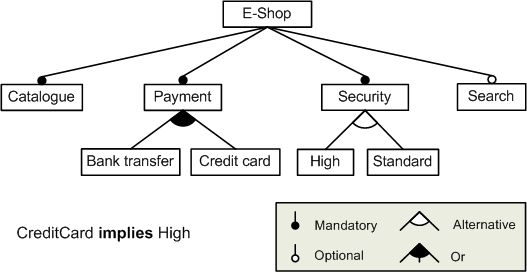
\includegraphics[width=0.7\textwidth]{bilder/E-shopFM.jpg}
\caption{Darstellung eines Featurediagramms für ein konfigurierbares E-Shop System von Segura09 in der Wikipedia auf Englisch (Transferred from en.wikipedia) [Public domain], via Wikimedia Commons.}
\label{fig:fd}
\end{figure}

\subsection{Metamodell}

Die Analyse des Problemfelds und Modellierung der Merkmale soll in erster Linie die Grundlage für die Definition des Metamodells der Domäne liefern\,\cite[S. 200]{stahl2007}. 

\subsubsection{Definition}

Zur Beschreibung welche Mittel zur Definition eines bestimmten Modells zur Verfügung stehen kann man wiederum ein Modell definieren. Dieses, über dem beschriebenen Modell stehende Modell, nennt man Metamodell. Stahl und Voelter bezeichnen es als Beschreibung der möglichen Struktur von Modellen. Dazu zählen sie die Konstrukte der Modellierungssprache, auf welche Weise diese zueinander in Beziehung stehen, sowie vorhandene Regeln bezüglich der Gültigkeit bzw. Modellierung\,\cite[S. 59]{stahl2007}.

Ein Unified Modeling Language 2.0 (UML) Diagramm welches alle Java Sprachkonzepte, wie beispielsweise die Existenz von Klassen, Attributen und Instanzen, beschreibt, ist eine Darstellung für das Java Metamodell. Geschriebener Java Quelltext wäre somit eine Instanz dieses Modells, kann aber wiederum instanziiert werden. Handelt es sich nämlich um eine Definition einer Java Klasse, so können hiervon Objekte mit konkreten Werten existieren.

Es ist noch hervorzuheben, dass mit dem Begriff Metamodell nicht einfach nur eine Abstraktion gemeint ist. Die Silbe Meta kann hier als  \glqq die Definition von\grqq\ verstanden werden. Ein Modell kann ein anderes Modell abstrahieren in dem es beispielsweise Informationen auslässt, falls diese für ein Anwendungsfall nicht relevant oder implizit sind. Das ist im obigen Sinne dann jedoch noch kein Metamodell. Zu sagen ein Metamodell ist das Modell eines Modells, ist also nur bedingt sinnvoll\,\cite[S. 27]{voelter2013}.

\subsubsection{Abstrakte Syntax und Konkrete Syntax}

Die in diesem Beispiel definierten Sprachkonzepte sind die abstrakte Syntax für Java. In Abgrenzung hierzu dient eine konkrete Syntax zur Beschreibung eines Modells. Möchte man einen Datentypen definieren, könnte man das mit einem UML Klassendiagramm. Da man den Datentypen auch mit Java-Code beschreiben könnte, sieht man, dass es für dasselbe Metamodell mehr als eine konkrete Syntax geben kann.\,\cite[S. 59f.]{stahl2007}.

\subsection{Domänenspezifische Sprache (DSL)}

Wurde das Metamodell für eine Domäne definiert, also ist die abstrakte Syntax bekannt, wird eine Möglichkeit benötigt eine Instanz des Metamodells zu bilden. Durch anreichern des Modells mit Informationen wird eine konkrete Ausprägung des Metamodells geschaffen. Das Mittel hierfür ist eine domänenspezifische Programmiersprache.

\subsubsection{Definition}

Stahl und Völter definieren eine solche Programmiersprache mit:\,\cite[S. 30]{stahl2007}. \glqq Eine DSL ist nichts anderes als eine Programmiersprache für eine Domäne.\grqq Martin Fowler hat in seinem Buch zu diesem Thema eine umfangreichere Definition geschaffen und erläutert diese mit vier Schlüsselelementen\,\cite[S. 27f.]{fowler2010}.

\begin{quote}\glqq Domain-specific Language (noun): a computer programming language of limited expressiveness focused on a particular domain.\grqq \end{quote}

Der Ausdruck \glqq Computer programming language\grqq\ bedeutet, dass eine DSL vom Menschen verwendet wird um einem Computer Befehle zu geben. Also sollte sie wie jede moderne Programmiersprache durch ihre Struktur sowohl vom Menschen leicht verständlich als auch vom Computer ausführbar sein.

Laut Fowler ist ein weiteres Element die \glqq Language nature\grqq. Als Programmiersprache sollte die Ausdrucksstärke einer DSL nicht nur von den einzelnen Ausdrücke kommen, sondern auch wie die Ausdrücke zusammengesetzt werden. 

Mit \glqq Limited expressiveness\grqq\ meint Fowler, dass eine DSL im Vergleich zu allgemeinen Programmiersprachen nur das für die Beschreibung der Domäne notwendige Minimum an Funktionalität aufweist. 

Im letzten Teil seiner Ausführung zu dieser Definition geht Fowler auf den \glqq Domain focus\grqq\ ein. Eine beschränkte Sprache sei nur sinnvoll wenn sie klar auf eine Domäne eingegrenzt ist.

\subsubsection{General Purpose Language (GPL)}

Die von Fowler angesprochenen allgemeinen Programmiersprachen bezeichnet man als General Purpose Language oder auch abgekürzt als GPL. Im Gegensatz zu DSLs sind GPLs nicht auf eine bestimmte Domäne zugeschnitten, sondern können breiter eingesetzt werden. Moderne Programmiersprachen wie Java und C\# sind solche Universalsprachen. Durch ihre Turing Vollständigkeit, kann man sie untereinander austauschen\,\cite[S. 111]{hromkovic2014}. Mehr als eine GPL gibt es, da sich einzelne Sprachen durch zusätzliche besondere Sprachfeatures voneinander abheben\,\cite[S. 27]{voelter2013}. Durch die Unterstützung von Pointern in C ist es zum Beispiel potenziell möglich Datenstrukturen besonders speicheroptimiert anzulegen\,\cite[S. 93ff.]{kernighan1988}.

\subsubsection{Interne DSLs}

Bettet man die Befehle zur Beschreibung einer Instanz des Metamodells auf geeignete Weise in eine Universalsprache ein, kann man dies interne DSL nennen. Der Aufbau und die Folge von Befehlen soll sich bei einer internen DSL, soweit möglich, wie eine eigene Sprache anfühlen\,\cite[S 28]{fowler2010}.

Für die Implementation von internen DSLs eignen sich dynamisch zu bezieht Sprachen wie Ruby und Lisp gut, da sie hilfreiche Features wie die Definition von Makros unterstützen. Je mehr in die normale Syntax einer Sprache eingegriffen werden kann, desto eigenständiger lässt sich die Syntax der internen DSL formen\,\cite[S. 98]{stahl2007}. Hierdurch grenzt sich diese immer weiter von einem einfachen application programming Interface (API) ab. Gerade wenn das Metamodell bei objektorientierter Programmierung in Form von Klassen vorliegt, kann eine interne DSL eher wie eine einfache Schnittstelle wirken. Die Abgrenzung von internen DSLs zu APIs ist nicht eindeutig und stellt eine Grauzone dar\,\cite[S. 67]{fowler2010}.

Eine erwähnenswerte Sonderform der intern DSLs sind fragmentierte DSLs. Bei diesem Spezialfall wird die Hostsprache, also die Programmiersprache mit der die interne DSL ausgedrückt wird, an einzelnen Stellen mit Informationen angereichert. Reguläre Ausdrücke die als Bruchstücke in einer GPL verwendet werden kann man hier als Beispiel anführen\,\cite[S. 32]{fowler2010}.

\subsubsection{Externe DSLs}

Eine externe DSL hat genau wie eine GPL eine eigene Syntax, laut Fowler ist es jedoch auch nicht unüblich dass die Syntax einer anderen Sprache, beispielsweise XML,  verwendet wird. Sprachen wie die Structured Query Language (SQL) oder Cascading Style Sheets (CSS) sind externe DSLs\,\cite[S. 28]{fowler2010}. SQL erlaubt es mit syntaktisch einfachen Mitteln Anfragen an eine Datenbank zu schicken und mit CSS kann die grafische Repräsentation von HTML-Seiten manipuliert werden.

Im Gegensatz zu internen DSLs, welche auf der Struktur der zugrunde liegenden GPL beruhen, erlauben externe DSLs ihre Syntax weitestgehend frei zu gestalten. Für ihre Implementation kann grundsätzlich auf einen reichen Schatz an Techniken, die zum verarbeiten von Programmiersprachen seit Jahren verwendet werden, zugegriffen werden\,\cite[S. 89]{fowler2010}.

\subsubsection{Language Workbenches}

Martin Fowler nennt bei der Kategorisierung von DSLs noch eine weitere, dritte Kategorie. Diese Language Workbenches sind hochspezialisierte Entwicklungsumgebungen zur Definition domainspezifischer Sprachen. Zusätzlich zu der Fähigkeit in einer solchen Entwicklungsumgebung DSLs zu definieren, dienen sie auch als Entwicklungsumgebung zur Verwendung dieser Sprachen\,\cite[S.28]{fowler2010}.

\subsection{Parser}

Ein großer Unterschied zwischen internen und externen DSLs besteht in ihrer Verarbeitung. Während interne DSLs eine Datenstruktur direkt mit Informationen befüllen, muss ein Ausdruck einer externen DSL, genau wie bei einem Ausdruck einer GPL, zuerst auf seinen semantischen Informationsgehalt analysiert werden.

\subsubsection{Einlesen des Quelltextes}

Normalerweise liegt der Quelltext, wie der Name schon sagt, in Textform vor. Wenn im folgenden von Quelltext die Rede ist so ist damit der Source Code von externen DSLs sowie der von GPLs gemeint. 

Zur Verarbeitung liest ein Reader den Quelltext zuerst ein und meist wird dieser dann in einem ersten Schritt zeilenweise von einem Lexer in seine Bestandteile (Token) zerlegt. Diese aufgespaltenen Code Zeilen können dann auf syntaktische Korrektheit geprüft werden und in eine Übergangsrepräsentation überführt werden\,\cite[S. 29f.]{parr2009}. Eine Form hierfür kann ein Abstract Syntax Tree (AST) sein.

\begin{figure}[htbp]
	\centering
	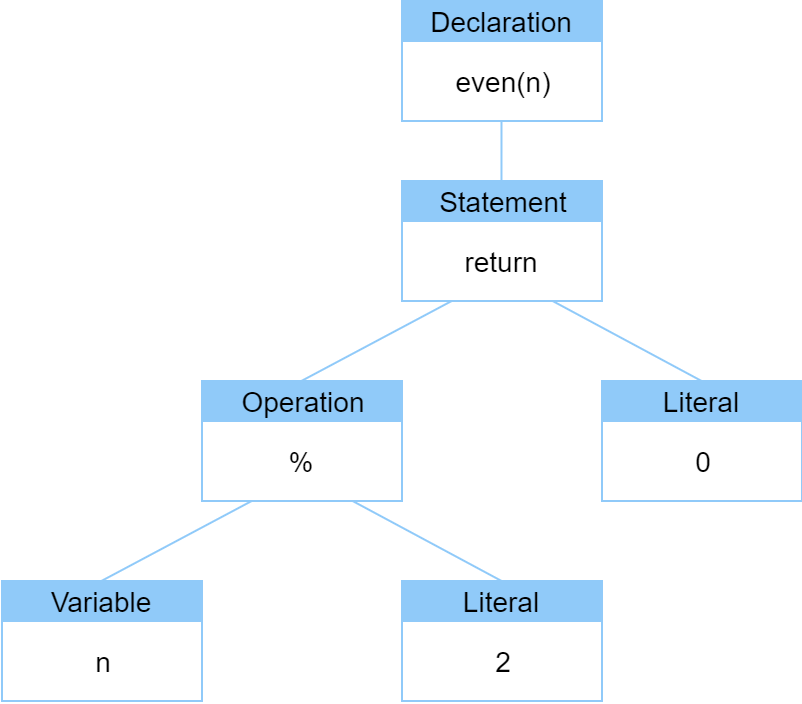
\includegraphics[width=1.0\textwidth]{bilder/ast}
	\caption{Darstellung einer Methode zur Prüfung der Parität einer natürlichen Zahl als AST}
	\label{fig:ast}
\end{figure}

\subsubsection{Abstract Syntax Tree (AST)}

Für jeden wichtigen Token wird im AST ein Knotenpunkt, mit für den weiteren Prozess wichtigen Daten, angelegt\,\cite[S. 23]{parr2009}. Die grafische Darstellung  des AST für die Prüfung der Parität einer natürlichen Zahl auf Abbildung ~\ref{fig:ast} zeigt diese Knoten-basierte Strukturierung des eingelesenen Codes. Die Knoten eines AST kennen ihre eigene Position im Baum und somit kann dieser mit geeigneten Strategien durchlaufen werden\,\cite[S. 24]{parr2009}.

Eine Möglichkeit ist die Anwendung des Visitor Patterns, welches in dieser Arbeit in einem späteren Unterkapitel der Grundlagen behandelt wird.

\subsubsection{Weitere Verarbeitung des eingelesenen Quelltextes}

Nachdem die syntaktische Korrektheit des Quelltextes sichergestellt ist und dieser in einer geeigneten Datenstruktur vorliegt, stehen jetzt mehrere Möglichkeiten zur Verfügung. Die jetzt in Baumstruktur vorliegenden Anweisungen sind jetzt durch Interpretation von einer Plattform ausführbar. Alternativ könnte auch eine Übersetzung in eine andere Sprache vorgenommen oder direkt zu ausführbaren Maschinencode kompiliert werden.

Bei Java wird der Quelltext beispielsweise eingelesen und zu Byte-Code transformiert, welcher dann von der Java Virtual Machine (JVM) interpretiert werden kann\,\cite{javavm2014}. Die Übersetzung in eine andere Sprache bietet sich sowohl bei externen DSLs als auch bei GPLs an. Allgemein könnte diese Transformation sinnvoll sein, wenn man seinen Code für eine bestimmte Plattform kompatibel zu einer anderen Plattform machen möchte. Ein Beispiel hierfür ist der Kompilierprozess einer in C\# geschriebenen Unity3D Anwendung zu einer WebGL App. Hierbei wird der C\# Code zuerst in C++ und dann in JavaScript umgewandelt\,\cite{unity2018}. Native GPLs wie C werden direkt zu Maschinensprache kompiliert\,\cite{kernighan1988}. Externe DSLs werden von einem Generator häufig zu GPL Quelltext transformiert\,\cite[S. 26]{voelter2013}.

\subsection{Code Generator}

Soll der vom Parser eingelesene Quelltext oder das von einer DSL beschriebene Modell nicht interpretiert, d. h. als Anweisungen an den Computer ausgeführt werden, kann ein Code Generator zum Einsatz kommen.

\subsubsection{Definition}

Nach Czarnecki und Eisenecker ist ein Generator ein Programm welches eine Spezifikation von Software auf einer höheren abstrakten Ebene entgegennimmt und dessen Implementation als Artefakt ausgibt\,\cite[S. 333]{czaeis2000}.

Das ausgegebene Artefakt kann, muss aber nicht zwingend, ein gesamtes lauffähiges Softwaresystem sein. Es könnten auch nur einzelne Klassen oder Funktionen generiert werden\,\cite[S. 333]{czaeis2000}. Sogar in einem noch kleineren Scope kommt Codegenerierung zum Einsatz, integrierte Entwicklungsumgebungen, wie JetBrains IntelliJ oder Microsofts Visual Studio, erlauben es auf Knopfdruck Code Snippets, wie zum Beispiel Konstruktoren für eine Klasse, zu generieren.

In der modellgetriebenen Softwareentwicklung dreht sich der gesamte Automatisierungsprozess um das Modell. Es bildet den Ausgangspunkt jeder weiteren Umwandlung. Wie bereits im Abschnitt zu MDSD beschrieben, sollen Änderungen nur am zugrunde liegenden Modell vorgenommen werden und nicht an hieraus entstandenen Generaten. Der Einsatz eines Codegenerators setzt dieses Vorgehen jedoch nicht zwingend voraus.

\subsubsection{Techniken zur Generierung von Code}

Herrington teilt Codegeneratoren in seinem Buch Codegeneration in Action in die zwei Hauptkategorien aktiv und passiv ein\,\cite[S. 28]{herrington2003}. 

Passive Codegeneratoren werden eingesetzt um einmal Quelltext zu generieren, zum Beispiel zur Unterstützung des Programmierers in einer integrierten Entwicklungsumgebung. Der Programmierer verarbeitet diesen generierten Code dann nach Belieben weiter. Im Gegensatz hierzu stehen aktive Codegeneratoren, welche immer wieder zur Ausführung kommen und den generierten Quelltext, abhängig von den Eingabeparametern des Generators, immer wieder regenerieren. Die für MDSD verwendeten Generatoren kann man dieser Kategorie zuordnen, die Eingabeparameter sind hier das konkrete Modell. 

Im Zusammenhang mit MDSD gibt es zwei Möglichkeiten der Generierung von Code aus dem konkreten Modell. Fowler nennt diese zwei Formen der Generierung Transformer Generation und Templated Generation\,\cite[S. 124f.]{fowler2010}.

Bei der Transformer Generation werden aus einem konkreten Modell Statements einer Zielsprache generiert. Hierfür wird das Modell traversiert und der Generator setzt aus den im Modell vorliegenden Informationen zum Aufbau des Codes Ausdrücke zusammen. Templated Generation basiert auf Textersetzung. Es wird eine Codevorlage, das Template, geschrieben in welcher Variabilitäten auf besondere Weise markiert sind. Aus den Daten des konkreten Modells werden konkrete Werte für diese Variabilitäten vom Generator ausgelesen und im Template eingesetzt.

Diese Ansätze sind nicht nur voneinander getrennt verwendbar. Beim Einsatz von Transformer Generation ist es denkbar, dass der Ausgabe Quelltext zwar komplett neu generiert wird, aber einzelne Teile dieses Quelltextes auf Basis von kleinen Templates erstellt werden\,\cite[S. 125]{fowler2010}.

\subsubsection{Zusammenhang mit Transformatoren}

Es ist denkbar ein von einer DSL beschriebenes Modell durch weitere Umwandlungsschritte weiter zu verarbeiten, bevor abschließend Quelltext generiert wird. Dies kann Sinn machen um ein Modell so aufzubereiten, dass ein bestimmter Generator es verarbeiten kann\,\cite[S. 195]{stahl2007}. Eine Komponente die diese Transformation durchführt nennt man Transformator. Wird ein Modell zu Text transformiert, so nennt man das Code Generierung, durchgeführt von einem Generator\,\cite[S. 271]{voelter2013}.

Ein konkreter Anwendungsfall wäre, wenn ein Generator, der eine konkrete Instanz eines bestimmten Metamodells zu Code verarbeiten kann, bereits implementiert vorliegt, jedoch das von einer DSL beschriebene Metamodell von dem für den Generator verständlichen Metamodell abweicht. Eine Modell zu Modell Transformation könnte hier eine Brücke schlagen und somit den bereits vorhandenen Generator nutzbar machen. Dies könnte unter Umständen, vor allem wenn die Metamodelle bereits eine ähnliche Struktur aufweisen, den Arbeitsaufwand reduzieren.

%%%%%%%%%%%%%%%%%%%%%%%%%%%%%%%%%
Die Komplexität der Umwandlung von einem Metamodell ins andere könnte durch mehrere Zwischentransformationen reduziert werden. Ein denkbarer Extremfall hierfür wäre die Reduktion der Transformationen auf nur eine einzelne Transformationsregel pro Modell Transformations Schritt.
%%%%%%%%%%%%%%%%%%%%%%%%%%%%%%%%%

\subsubsection{Abgrenzung zu Compilern}

In der Literatur wird ein Generator stellenweise auch Compiler\,\cite[S. 26]{voelter2013} bzw. Code generieren auch kompilieren genannt\,\cite[S. 19]{fowler2010}.

Jedoch kann man bei genauerem hinsehen Generatoren von Compilern im Zusammenhang mit MDSD voneinander gut abgrenzen. Bei der modellgetriebenen Softwareentwicklung wandeln Generatoren DSL Code in konkreten Code einer GPL um. Normalerweise wird aus DSL Code nicht direkt Bytecode oder Maschinencode generiert, da wir durch den Schritt über GPL Code den Compiler der GPL mit all seinen Features verwenden können\,\cite[S. 11]{voelter2013}.
	
Wie beschrieben, wandelt ein Compiler GPL Code zu Bytecode oder Maschinencode um. Dabei nimmt er Optimierungen wie zum Beispiel zur Verbesserung der Geschwindigkeit oder des Speicherverbrauchs eines Programms vor. Das vom Compiler erzeugte Artefakt kann auf der Zielplattform direkt ausgeführt werden\,\cite[S. 345ff.]{czaeis2000}.
	
Da eine Beschreibung des Kompilierprozesses und die verwendeten Techniken im Compilerbau den Rahmen dieser Arbeit sprengen würden, wird hier nicht tiefer auf das Thema eingegangen, sondern auf das \glqq Drachenbuch\grqq\ als weiterführende Literatur verwiesen\,\cite{aho2006}.

\section{Software Engineering}

Software Engineering, auch bekannt unter der deutschen Bezeichnung Softwaretechnik, wird von Helmut Balzert in seinem Lehrbuch der Softwaretechnik folgendermaßen definiert\,\cite[S.17]{balzert2009a}:

\begin{quote}
	Softwaretechnik: Zielorientierte Bereitstellung und systematische Verwendung von Prinzipien, Methoden und Werkzeugen für	die arbeitsteilige, ingenieurmäßige Entwicklung und Anwendung von umfangreichen Softwaresystemen. Zielorientiert bedeutet die	Berücksichtigung z. B. von Kosten, Zeit, Qualität.
\end{quote}

Also geht es um die wirtschaftliche Anwendung von erprobten Lösungen bei der Umsetzung großer Softwaresysteme. Außerdem soll dies systematisch geschehen, es soll begründet werden wieso ein Prinzip, eine Methode oder ein Werkzeug zur Lösung eines bestimmten Problems verwendet wurde. In der Softwaretechnik geht nicht darum das Rad jedes Mal neu zu erfinden, der vorhandene Stand der Technik soll strukturiert angewandt werden.

Für den Bereich der Prinzipien in der Softwaretechnik hat Balzert einige grundlegenden Konzepte zusammengefasst und diese in Relation zueinander gestellt. Da diese Prinzipien einen wichtigen Teil der Softwareentwicklung ausmachen und für diese Arbeit systematisch eine Software entwickelt wurde, sind diese auch hier sehr relevant.

\subsection{Prinzipien der Softwaretechnik}

Ein Prinzip liegt als Basis dem zugrunde was wir tun. Sie sind weder konkret, noch beziehen sie sich auf Spezialfälle\,\cite[S. 25]{balzert2009a}. 

\subsubsection{Abstraktion}

Abstrahieren bedeutet etwas zu verallgemeinern, d. h. sich von besonderen Eigenschaften einer Sache zu lösen und wesentliche Dinge und gleiche Merkmale die mehrere Instanzen dieser Sache haben hervorzuheben. Im Gegensatz zur Abstraktion steht die Konkretisierung\,\cite[S. 26]{balzert2009a}.

In der Softwareentwicklung ist eine Form der Abstraktion der Aufbau von Vererbungsstrukturen in der objektorientierten Programmierung. Hier werden allgemeine Eigenschaften in eine Oberklasse abstrahiert und andere Klassen erben hiervon und fügen eigene, spezielle Eigenschaften hinzu.

Abstraktion und Modellbildung treten häufig gemeinsam auf. Möchte man in einer Anwendung beispielsweise Personen verwalten, so ist es kaum möglich alle Eigenschaften die eine reale Person mitbringt als Modell abzubilden. 

Bei einer Kundenverwaltung sind für eine Anwendung vermutlich Attribute wie der Name, das Passwort und die Adresse eines Kunden relevant. Zusätzliche Merkmale dieser Person, wie zum Beispiel die die Haarfarbe werden nicht abgebildet. Der Grund hierfür könnte sein, dass dies für eine Kundenverwaltung nicht relevant ist, die Haarfarbe wurde abstrahiert.

Selbst wenn ein Modell so genau wie möglich sein soll, muss an einer Stelle ein Schlussstrich gezogen werden. Die Haarfarbe mag relevant sein, also könnte man hier für die Haarfarbe rot oder blond abbilden, aber dies ginge noch genauer, man könnte noch Abstufungen unterscheiden. Vielleicht sollte man Haarfarbe an sich noch genauer festhalten, denn die Frage aus welchen rot, grün und blau Werten sich die Farbe genau zusammensetzt bleibt trotzdem noch offen. Abstraktion ist also irgendwann notwendig.

\subsubsection{Modularisierung}

Im direkten Zusammenhang mit Abstraktion steht das Prinzip der Modularisierung. Modularisierung bedeutet ein System in Module zu zerlegen. Dieses Konzept kommt zum Beispiel besonders häufig bei Elektrogeräten vor. Ein Computer hat mehrere, einzeln entwickelte, Bauteile. Der Arbeitsspeicher ist von einem anderen Hersteller als die Grafikkarte. Über eine definierte Schnittstelle, die Anschlüsse auf der Hauptplatine, können Arbeitsspeicher und Grafikkarte gemeinsam in einem System betrieben werden.

Ein Modul stellt eine funktionale Einheit oder eine auf semantische Weise verbundenen Funktionsgruppe dar. Ebenso ist ein Modul weitgehend Kontext unabhängig, d. h. es kann für sich stehend verstanden, entwickelt, geprüft und gewartet werden. Gekoppelt sind die Module über eine klar erkennbare Schnittstelle\,\cite[S. 41]{balzert2009a}.

\subsubsection{Weitere Prinzipien und Abhängigkeiten zwischen den Prinzipien der Softwaretechnik}

Es gibt neben den genannten Prinzipien noch einige weitere die hier nicht tiefer behandelt werden. Das Prinzip der Strukturierung besagt, dass ein Softwaresystem in einer bestimmten definierten Struktur vorliegt\,\cite[S. 34ff.]{balzert2009a}. Bindung und Kopplung beschreiben strukturelle Eigenschaften eines Softwaresystems. Bindung bezeichnet hierbei die Kompaktheit einer Systemkomponente. Ist ein System stark gebunden, so haben die einzelnen Komponenten ihre klar definierten Verantwortlichkeiten. Im Gegensatz zur Bindung steht die Kopplung, diese ist die Assoziation und Vererbungsstruktur zwischen verschiedenen Klassen und Paketen. Je höher der Kopplungsgrad ist, desto größere Auswirkungen haben Änderungen in einer Komponente auf andere, hiermit gekoppelte, Komponenten\,\cite[S. 37f.]{balzert2009a}. Wenn ein System nach einer Rangordnung angeordnet ist, so besitzt es eine Hierarchie. Dies ist eine stärkere Form der Strukturierung und verhindert es, dass ein Softwaresystem eine chaotischer Struktur entwickelt\,\cite[S. 39ff.]{balzert2009a}. Unter Geheimnisprinzip versteht man eine schärfere Version der Modularisierung, für ein Anwender soll eine Systemkomponente keinen Einblick in die eigene Funktionsweise bieten sondern nur korrekt funktionieren\,\cite[S. 42ff.]{balzert2009a}. Lokalität bedeutet, dass für eine Aufgabe wichtige Informationen nicht Zusammengesucht werden müssen, sondern zum Beispiel als Felder in einer Klasse bereits vorliegen\,\cite[S. 45f.]{balzert2009a}. Mit dem Prinzip der Verbalisierung ist unter anderem gemeint, dass Komponenten, wie Klassen, Methoden und Felder eine aussagekräftige Namensgebung haben, da dies bis zu einem gewissen Grad zu einer Selbstdokumentierung des Codes führt\,\cite[S. 46ff.]{balzert2009a}.

Die Prinzipien der Softwaretechnik stehen nicht losgelöst im Raum, sondern sie bedingen sich teilweise oder stehen zueinander in Wechselwirkung. Bindung und Kopplung benötigt zum Beispiel Modularisierung bzw. Strukturierung das Geheimnisprinzip kann auch nur auf Basis von Modularisierung Anwendung finden. Ein Graph der diese Zusammenhänge abbildet findet sich bei Balzert\,\cite[S. 49]{balzert2009a}.

\subsubsection{Zusammenhang zwischen den Prinzipien der Softwaretechnik und der Entwicklung von Codegeneratoren}

Wie bereits eingangs erwähnt, haben die in vorherigen Kapiten beschriebenen Prinzipien einen direkten Zusammenhang mit der Entwicklung von Codegeneratoren.

Insbesondere sticht die für die modellgetriebene Software Entwicklung unerlässliche Abstraktion durch Modellbildung heraus. Vor allem ein Metamodell stellt die Verallgemeinerung der relevanten Konzepte eine Domäne dar. Eine verwendete DSL zur Beschreibung des Metamodells abstrahiert demnach Konzepte einer GPL oder einer Domäne.

Modularisierung findet bei MDSD durch die Einteilung der einzelnen Arbeitsschritte in einzelne Softwarekomponenten statt. Ein Metamodell hat eine definierte abstrakte Syntax, eine hieraus gebildete konkrete Syntax ist eine Schnittstelle für das Modul Metamodell. Ein Parser als weitere Komponente liest eigenständig Quelltext ein und bildet diesen auf einen AST ab. Mit einer Schnittstelle kann der eingelesen Quelltext weiterverarbeitet werden. Codegenerator ist hier unabhängig vom konkret gewählten Parser, er verarbeitet nur den AST und ein anderes aus dem Parsing Prozess hervorgegangenes Modell. Auch für den Parser ist es nicht relevant wie der einzulesende Quelltext entstanden ist, er muss lediglich syntaktisch korrekt sein.

\section{Design Pattern objektorientierter Programmierung}

Das viel beachtete Werk Design Patterns: Elements of Reusable Object-Oriented Software stellt einen Katalog auf, welcher Beschreibungen für Muster liefert die allgemeine Designprobleme in ein bestimmten Kontext lösen\,\cite{gamma1995}. Diese Muster, von den Autoren des Werks Pattern genannt, haben grundsätzlich vier Elemente: 

Zum einen der Name welcher verwendet werden kann um auf das Pattern zu referenzieren. Dies ermöglicht, allein schon durch die Erweiterung des Vokabulars, Software mit erhöhter Abstraktion zu entwerfen. Zum anderen gehört zu jedem dieser Muster eine Beschreibung bei welcher Art von Problem es anwendbar sein könnte. Als dritter Teil eines Patterns werden die Elemente, welche verwendet werden um das beschriebene Problem zu lösen, abstrakt beschrieben. Diese Lösungen beschreiben kein konkretes Design oder eine konkrete Implementation da das Muster in verschiedenen Situation Anwendung finden kann. Jedes Muster bringt Vor- und Nachteile, diese Konsequenzen sind wichtig zum Verständnis eines Patterns und sollten daher explizit aufgeführt werden\,\cite[S.30 f.]{gamma2015}.

Modellgetriebene Software Entwicklung stellt uns im Zusammenhang mit objektorientierter Programmierung vor Probleme für welche bestimmte Design Pattern hilfreich sein können. Die Beschreibung dieser Entwurfsmuster folgt in dem oben zitierten Werk einem konsistenten Aufbau. Die folgenden Abschnitte dieser Arbeit orientieren sich an dieser Vorlage. Erst wird das Pattern benannt, dann wird kurz der Zweck, also was mit der Verwendung des Patterns erreicht werden soll, zusammengefasst. Dies wird gefolgt von einer Erklärung wann das Pattern anwendbar sein könnte und zum Abschluss wird in Form eines Diagramms das behandelte Muster dargestellt. Erklärungen zur verwendeten Notation können auf den ersten Seiten der aktuellen deutschen Übersetzung des Design Pattern Werkes entnommen werden\,\cite[S. 8]{gamma2015}. Der genaue Aufbau und der Ablauf der Kommunikation zwischen den Akteuren des Patterns wird in dieser Arbeit nur oberflächlich erläutert. Die Intention dieses Abschnitts ist, dass die aufgezeigten Muster, wenn diese später erwähnt werden, in ihrer grundlegenden Funktion bekannt sind.

Das Factory Method Pattern bezeichnet hier nicht das von Gamma et al. vorgeschlagene Factory Method Muster\,\cite[S. 173ff.]{gamma2015}, sondern bezieht sich auf die von Bloch in Effective Java beschriebene Static Factory Method\,\cite[S. 5ff.]{bloch2017}.

\subsection{Visitor Pattern}

Das Visitor Pattern oder auch Besuchermuster ist ein objektbasiertes Verhaltensmuster\,\cite[S. 480]{gamma2015}.

\subsubsection{Zweck}

Dieses Muster erlaubt es Operationen auf Elementen einer Objektstruktur zu definieren, ohne die eigentlichen Klassen der Elemente ändern zu müssen\,\cite[S. 480]{gamma2015}.

\subsubsection{Anwendbarkeit}

Das Besuchermuster kann sinnvoll Anwendung finden wenn eine Struktur aus Objekten mit unterschiedlichen Schnittstellen vorliegt und auf diesen Objekten, abhängig von ihrer konkreten Klasse, Operationen auszuführen sind. Dies schützt vor allem davor, dass die Klassen dieser Objekte für jede Anwendung die jeweiligen Operationen implementieren müssen. Wird die Objektstruktur verwendet so können die notwendigen Operationen lokalisiert definiert werden. Das Besuchermuster erlaubt es leicht neue Operation hinzuzufügen, sollte sich jedoch die Objektstruktur häufiger ändern, so müssen jedes Mal die Visitor Schnittstellen neu definiert werden. Hier könnte es besser sein die Operationen in den betroffenen Klassen zu definieren\,\cite[S. 484]{gamma2015}.

Ein Anwendungsbeispiel für das Visitor Pattern bei modellgetriebener Softwareentwicklung ist die Verarbeitung der Nodes eines AST. Der Baum stellt hier die erwähnte Objektstruktur dar und dessen Knoten die Elemente\,\cite[S. 480]{gamma2015}.

\subsubsection{Struktur}

Abbildung ~\ref{fig:visitor} zeigt den Aufbau des Visitor Patterns. Sind die entsprechenden Klassen auf diese Weise implementiert, so kann jederzeit, wenn eine Operation auf den Elementen einer Datenstruktur ausführbar gemacht werden soll, ein konkreter Visitor implementiert werden welcher diese Operation ausführt. Traversiert man die einzelnen Objekte der Struktur, kann auf jedem dieser Objekte die Accept Operation aufgerufen werden. Diese führt dann die entsprechende Visit Operation auf dem übergebenen konkretenen Visitor aus. Es ist möglich, dass nicht eine einzigartig benannte Visit Operation für jedes konkrete Element existiert, sondern, dass die Operation durch Funktionsüberladung einer aussagekräftig benannten Visit()-Methode implementiert wird\,\cite[S.485 ff.]{gamma2015}.

\begin{figure}[htbp]
	\centering
	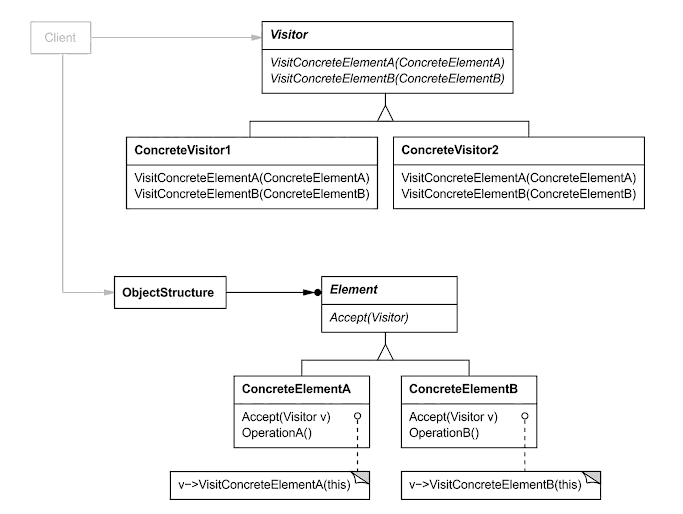
\includegraphics[width=1.0\textwidth]{bilder/visitor}
	\caption{Darstellung der Struktur des Visitor Design Patterns, entnommen aus\,\cite[S. 485]{gamma2015}.}
	\label{fig:visitor}
\end{figure}

\subsection{Builder}

Das Pattern Builder oder im deutschen auch Erbauer ist ein objektbasiertes Erzeugungsmuster\,\cite[S. 159]{gamma2015}.

\subsubsection{Zweck}

Ein Erbauer soll die Erzeugung eines komplexen Objektes von dessen Repräsentation trennen. Somit ist es möglich unterschiedlich aufgebaute Instanzen einer Klasse zu erzeugen\,\cite[S. 159]{gamma2015}. Eine spezielle Form des Builders, die Joshua Bloch in Effective Java vorschlägt, dient dazu komplexe Objekte mit vielen optionalen Parametern vereinfacht zu konstruieren\,\cite[S. 10ff.]{bloch2017}. 

\subsubsection{Anwendbarkeit}

Soll die Logik die bei der Erzeugung eines komplexen Objektes verwendet wird losgelöst sein von dem eigentlichen Objekt oder soll das komplexe Objekt optionale Parameter ermöglichen, könnte man einen Builder verwenden.

Ein Anwendungsfall für die Verwendung eines Builders stellt die Implementation einer internen DSL dar. Das beschriebene komplexe Objekt ist hier die konkrete Instanz des Metamodells\,\cite[S. 343ff.]{fowler2010}.

\subsubsection{Struktur}

Wie bei vielen der von Gamma et al. beschriebenen Pattern, definiert eine Abst rakte Klasse eine Schnittstelle mit den zur Erzeugung verwendbaren Methoden, welche dann von einer konkreten Klasse implementiert werden. Hier sind das die Klassen Builder und ConcreteBuilder. Ein Director verwendet diese Schnittstelle und erzeugt damit ein konkretes Produkt\,\cite[S. 162f.]{gamma2015}. Eine mögliche Abwandlung davon wäre die von Bloch beschriebene Erweiterung der BuildPart() Methoden um eine Referenz auf das aktuelle Builder Objekt als Rückgabewert. Der Builder hält den aktuellen Zustand des erzeugten Objekts und erst wenn bei der dadurch entstehenden Methodenkaskade eine abschließende Build() Methode aufgerufen wird, gibt der Builder das erzeugte Objekt zurück\,\cite[S. 13ff]{bloch2017}.

\begin{figure}[htbp]
	\centering
	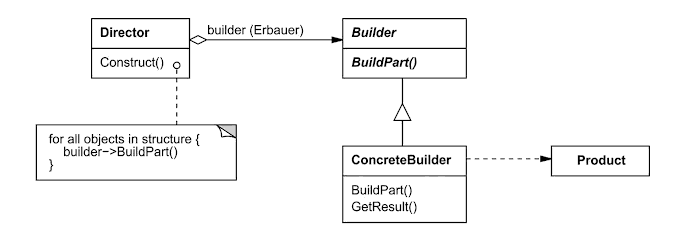
\includegraphics[width=1.0\textwidth]{bilder/builder}
	\caption{Darstellung der Struktur des Builder Design Patterns, entnommen aus\,\cite[S. 162]{gamma2015}.}
	\label{fig:builder}
\end{figure}

\subsection{Factory Method}

Obwohl die Factory Method, oder auch Fabrikmethode, in dieser Form nicht von Gamma et al. in ihrem Katalog beschrieben wurde, könnte man sie als ein objektbasiertes Erzeugungsmuster bezeichnen, da sie ebenfalls Objekte einer Klasse instanziiert.

\subsubsection{Zweck}

Ziel einer Factory Method ist es, anstelle von speziellen Konstruktoren,  statische Methoden zur Erzeugung von Objekten bereitzustellen. Da eine Methode im Gegensatz zu Konstruktoren benannt werden kann, ist es möglich die erzeugte Instanz eindeutiger zu beschreiben\,\cite[S. 5f]{bloch2017}. 

\subsubsection{Anwendbarkeit}

Die Verwendung von Fabrikmethoden kann sinnvoll sein wenn die Parameter eines Konstruktors das erzeugte Objekt nicht eindeutig beschreiben. Hier kann eine sprechend benannte statische Fabrikmethode eine genauere Beschreibung bieten und die Lesbarkeit des Quelltextes erhöhen. Es ist nicht möglich Konstruktoren mit gleicher Signatur aber unterschiedlichem Verhalten bereitzustellen, statische Fabrikmethoden können solche Konstruktoren ersetzen. Statische Fabrikmethoden können Objekte eines Subtypen zurückgeben, somit kann die eigentliche instanziierte Klasse versteckt werden\,\cite[S. 5ff]{bloch2017}.

In Verbindung mit einem Enum oder String als Parameter der statischen Fabrikmethode, kann die Erzeugung eines komplexen Objekts mit einer aussagekräftigen Benennung gesteuert werden.

Eine Möglichkeit zur Erzeugung eines Generats ist die Zusammenstellung aus Komponenten. Man könnte statische Methoden zur Erstellung der jeweiligen Komponenten verwenden.

\subsubsection{Struktur}

Da es für die statische Fabrikmethode nach Bloch kein Gegenstück im Katalog Design Pattern Gamma et al. existiert\,\cite[S. 5]{bloch2017} und die Struktur lediglich durch das Hinzufügen weiterer Methoden zu einem Objekt besteht, wird hier auf eine Abbildung verzichtet. 

Eine statische Fabrikmethode ist eine von außen zugängliche statische Methode einer Klasse mit beliebigen Parametern die, wie ein Konstruktor, ein Objekt dieser Klasse zurückgibt. Sie kann die Konstruktoren einer Klasse vollständig ersetzen oder die Klasse erweitern\,\cite[S. 5f]{bloch2017}. Die statische Fabrikmethode könnte auch in eine extra Fabrik Klasse ausgelagert werden um so Logik für die Instanziierung verschieden konfigurierter Objekte einer Klasse lokal zu Sammeln.

\chapter{Analyse}

\begin{quote}\glqq Wie kann, ausgehend von bestehendem Java-Code, die Entwicklung eines Generators zur Erhöhung der Wirtschaftlichkeit Modellgetriebener Softwareentwicklung automatisiert werden?\grqq \end{quote}

Auf Basis der Grundlagen ist es jetzt möglich diese Hauptfragestellung dieser Arbeit eingehend zu analysieren. Das folgende Kapitel wird zuerst auf einen Vergleich des Aufwands bei konventionellen Softwareprojekten und modellgetriebener Softwareentwicklung eingehen. Es soll klargemacht werden wo die wirtschaftlichen Hürden bei MDSD liegen. Der zweite Abschnitt dieser Analyse beschäftigt sich Schritt für Schritt mit den Schwierigkeiten die bei der Umsetzung eines Proof-of-Concept zur Beantwortung der obigen Fragestellung auftreten können.

Zu jedem analysierten Problem werden mögliche Lösungswege aufgeführt und ihre Vor- und Nachteile erörtert. Das Ziel dieses Abschnitts ist es, dass im nachfolgendem Konzept Kapitel auf diese Analyse zurückgegriffen werden kann und somit der im Konzept gewählte Ansatz begründ- und nachvollziehbar ist. Wenn in den folgenden Abschnitten im Zusammenhang mit Generierung und Automatisierung von Apps, Anwendungen und Produktfamilien die Rede ist, so ist dies beispielhaft gemeint. Die beschriebenen Probleme beziehen sich auch auf einen kleineren Skopus, zum Beispiel für Module oder Klassen, fallen in diesen Zusammenhängen aber entsprechend kleiner aus.

\section{Aufwand eines konventionellen Softwareprojektes im Vergleich zu MDSD}

Die Umsetzung einer Anwendung hat unterschiedliche Etappen. Zu Beginn der Entwicklung wird spezifiziert was entwickelt werden soll, also welche Anforderungen die Anwendung gestellt werden. Gefolgt von einer Entwurfsphase, in welcher beschrieben wird wie die Anwendung aussieht und aus welchen Bausteinen sie besteht. Als letzter Schritt wird das in Entwurfsphase erarbeitete Konzept implementiert\,\cite[S. 62]{balzert2009a}. Abhängig vom verwendeten Entwicklungsprozess, wird parallel zu dieser Entwicklung oder im Anschluss daran die Qualität der Anwendung durch Tests gesichert. Sind diese Etappen alle erledigt, kann die App veröffentlicht werden.

Die Idee der modellgetriebenen Software Entwicklung ist es, dass man vereinfacht und ab einem gewissen Punkt wirtschaftlich, ganze Anwendungen oder Teile derer einfacher, schneller und wiederverwertbar generieren kann\,\cite[S. 14f.]{stahl2007}. Ein Beispiel hierfür wäre die Umsetzung verschieden konfigurierter Ausprägungen einer Anwendung, basierend auf einer Softwarefamilie\,\cite[S. 237ff.]{stahl2007}. Wie aus den im vorherigen Kapitel beschriebenen Grundlagen hervorgeht, hat auch MDSD grundsätzlich mehrere Entwicklungsschritte. Um Software mit einem Modell beschreiben und daraus generieren zu können, muss bekannt sein wie diese Software aufgebaut ist und funktioniert. Ein erster Schritt bei MDSD kann also sein, eine Ursprungs App zu entwicklen, welche als Referenz für den weiteren Entwicklungsprozess dient. Danach kann diese Referenzimplementation analysiert werden. Hierunter fällt auch das in Grundlagen beschriebene Domain Engineering und die Definition eines Metamodells. Hierauf aufbauend kann zum einen eine domänenspezifische Sprache entwickelt werden, zum anderen ein Generator, welcher aus einer Instanz des Metamodells verschiedene Ausprägungen der Software generieren kann.

Bereits für die Umsetzung einer Referenzimplementation muss der gleiche Prozess durchlaufen werden, wie der für das konventionelle umsetzen einer App\,\cite[S. 219f.]{stahl2007}. Da bei MDSD noch eine umfangreiche Analysephase und die Entwicklung des Generators durchgeführt werden muss, kann modellgetriebene Softwareentwicklung sich frühestens mit der Entwicklung einer zweiten App einer Softwarefamilie oder vielleicht sogar erst zu einem späteren Zeitpunkt wirtschaftlich rechnen. Abbildung ~\ref{fig:vgl1} stellt diesen Vergleich grafisch vereinfacht dar.

\begin{figure}[htbp]
	\centering
	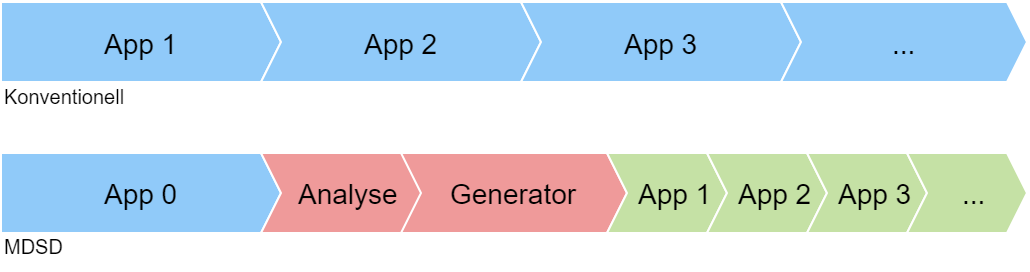
\includegraphics[width=0.9\textwidth]{bilder/vergleich_1}
	\caption{Vereinfachte Darstellung des Aufwandsvergleichs eines konventionellen Softwareprojektes und MDSD.}
	\label{fig:vgl1}
\end{figure}

Ein zusätzlicher Faktor der die Wirtschaftlichkeit von MDSD beeinträchtigen könnte ist, dass der Entwicklungsprozess bei der Verwendung eines modellgetriebenen Ansatzes ein Entwicklungsteam normalerweise aufteilt. Ein Teil der Entwickler erweitert DSLs und Generatoren und der andere Teil verwendet diese. Diese Abhängigkeit muss in der Ablaufplanung des Projektes berücksichtigt werden. Da sich bei MDSD nicht um konventionelle Softwareentwicklung handelt, kann es zusätzlich sein, dass die Konzepte einem Entwicklungsteam erst nähergebracht und etwaige Kompetenzen erst aufgebaut werden müssen\,\cite[S. 44ff.]{voelter2013}.

Betrachtet man den MDSD Entwicklungsprozess strukturiert von Anfang bis Ende, ist gut zu sehen an welcher Stelle eine Erhöhung der Wirtschaftlichkeit denkbar wäre. 

Das umsetzen einer Referenzimplantation kann, wie bereits beschrieben, kaum gekürzt werden. Eine vollständige Analyse ist nur möglich wenn auch eine zu analysierende Anwendung exisitiert. Da wir mit dem Generator konkreten Quelltext erzeugen wollen, reicht auch eine reine Konzeptionierung der Referenzimplementation kaum aus, sie sollte codiert vorliegen. Es könnte möglich sein mithilfe von zum Beispiel Feature Modelling den großteil einer Domäne losgelöst von einer konkreten Implementation zu analysieren. Spätestens wenn es darum geht die zu generierende Architektur zu untersuchen, ist die Referenzimplementierung eine wichtige Hilfestellung und Ausgangspunkt hierfür\,\cite[S. 123f.]{stahl2007}.

Da die Analyse der Domäne und die Entwicklung des Metamodells sich nicht nur auf die Referenzimplementation stützt, sondern sich auch auf semantische, in der Referenzimplementation nicht zwingend festgehaltene, Zusammenhänge bezieht, ist sie nur sehr schwer und wenn überhaupt nur in Teilen automatisierbar. 

Im Gegensatz dazu steht die geradezu mechanisch anmutende Generierung von konkretem Quelltext aus einer Instanz eines beschriebenen Metamodells. Ist durch die Referenzimplementation und Analyse bekannt wie die allgemeine Architektur für eine Anwendung aussieht und durch das Metamodell welche Variabilitäten vorliegen, so folgt die Erzeugung von Quelltext eindeutig vorher definierbaren Regeln. Konkrete Instanzen von Modellen die für einen solchen Generator verständlich sind, müssten also dann alle auf dem gleichen Metamodell beruhen. Eine DSL zur Instanziierung eines solchen Metamodells könnte dann entweder immer gleich aussehen oder davon abhängen welche Variabilitäten, basierend auf einer Referenzimplementation, überhaupt beschreibbar sein müssen. Unabhängig hiervon besteht in diesem Schritt somit Potenzial den MDSD Prozess durch Automatisierung zu verkürzen. Die folgende Abbildung ~\ref{fig:vgl2} zeigt dieses Potenzial in vereinfachter grafischer Darstellung noch einmal auf.

Der Aufwand des letzten Schritts, der eigentlichen Anwendung des Generators, hängt von den oben bereits erwähnten Kompetenzen der Entwickler und vor allem mit der zur Modellbeschreibung verwendeten DSL zusammen. Je einfacher die DSL verwendet werden kann, je eindeutiger und eingängig ihre Syntax und je stärker die durch die DSL ermöglichte Abstraktion ist, desto produktiver kann mit ihr gearbeitet werden. Um dies bei DSLs zu erreichen haben Stahl und Voelter einige Best-Practices zur Definition von DSLs formuliert\,\cite[S. 113]{stahl2007}. Einsparungen können hier also im Grunde nur im Vorfeld, also bei der Analyse unter Umsetzung des Generators ausgelöst werden. Welche Ausprägung einer Anwendung genau generiert werden soll, muss ein Entwickler immer noch manuell schreiben.

\begin{figure}[htbp]
	\centering
	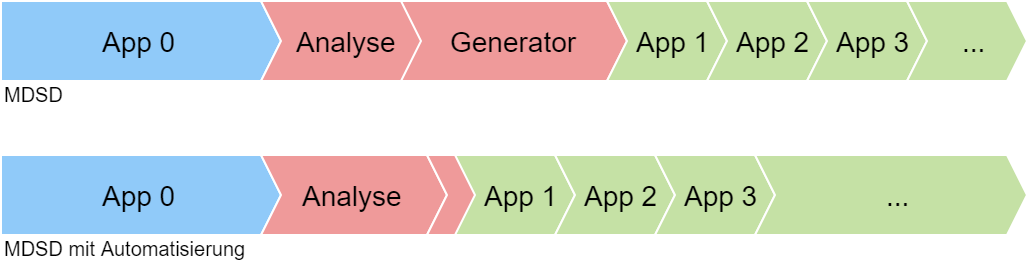
\includegraphics[width=0.9\textwidth]{bilder/vergleich_2}
	\caption{Vereinfachte Darstellung des Einsparungspotentials im Generator Implementations-Schritt bei MDSD.}
	\label{fig:vgl2}
\end{figure}


\section{Automatisierung der Entwicklung eines Code Generators}

Wie aus dem vorherigen Abschnitt entnommen werden kann, besteht ein großes Automatisierungspotenzial darin den gesamten Generator oder Teile davon automatisiert zu erzeugen, hierbei treten einige Schwierigkeiten auf, welche im folgenden genau analysiert werden. Im Rahmen dieser Arbeit wird davon ausgegangen, dass eine Referenzimplementation bereits in Form von Java Quelltext vorliegt.

\subsection{Java Code als Ausgangsmodell}

Um die existierende Referenzimplementation weiter verarbeiten und hieraus ableiten zu können welche Variabilitäten in Generaten auf Basis dieser Referenz existieren, müssen Informationen hierzu festgehalten und für den Metagenerator zugänglich gemacht werden. Das bedeutet, dass zum Beispiel zur Implementation einer Java Klasse zusätzlich die Informationen vorliegen muss, dass in einer generierten Variante dieser Klasse der Identifier variabel bestimmt werden kann.

\subsubsection{Anreicherung des Java Codes mit Informationen}

Es gibt mehrere Möglichkeiten zusätzliche Informationen zum vorhandenen Java Quelltext anzubringen. Ein Ansatz hierfür wäre dies als zusätzliches Modell, zum Beispiel in einer XML Datei\,\cite{xml2008}, zu formulieren. Hier könnten dann unter der Verwendung von XML Tags und Attributen Referenzen zu bestehenden Klassen gebildet werden. Beim einlesen des Java Quelltextes würde dann auch das zugehörige XML Dokument geparsed und nach korrespondierenden Informationen durchsucht werden. Mit XML Schema Definitions Dateien (XSD)\,\cite{xsd2012} und Unterstützung von geeigneten APIs wie JAXB\,\cite{jaxb} könnte sehr genau beschrieben werden wie dieses Modell aufgebaut sein dürfte. Alle Informationen zu Erweiterung einer Java Quelltext Datei wären an einer Stelle zu finden. Außerdem müsste ein Benutzer des Metagenerators, anstatt nur einzelne Stellen in seiner Referenzimplementation zu markieren, eine zusätzliche XML Datei nach den Regeln der zugehörigen XSD Datei aufstellen.

Als weiterer Ansatz könnten Stellen im Quelltext, die mit Informationen angereichert werden sollen, zeilenweise mit Kommentaren versehen werden. Die genaue textuelle Form der Kommentare ist hier frei wählbar. Also wäre es sogar denkbar eine hier eigenständige DSL zu verwenden. Der Informationsgehalt und dessen semantische Bedeutung müssten nach oder beim parsen des Java Quelltextes in einem zusätzlichen Schritt analysiert werden. Kommentare könnten an jeder Stelle des Codes, also auch innerhalb von Methoden, theoretisch sogar innerhalb von einzelnen Ausdrücken, verwendet werden. Eine Einschränkung welcher Kommentar an welche Stelle des Codes gesetzt werden darf kann jedoch nicht ohne zusätzliche Hilfsmittel gemacht werden.

Eine dritte Variante wäre es den Quelltext mit Java Annotationen zu versehen. Abhängig von der Information die eine solche Annotation anbringen soll, könnte eine semantisch passende Benennung gewählt werden. Durch zusätzliche Target Annotationen an den Annotations Definitionen könnte noch genauer bestimmt werden an welcher Stelle im Code welche Annotation angebracht werden darf. Mit Hilfe von Annotations Parameter könnten noch weitere Informationen übergeben werden. Da es nicht möglich ist Quelltext innerhalb von Methoden zu annotieren, könnten dort auf diesem Weg keine zusätzlichen Informationen angegeben werden.

\subsubsection{Parsen des Java Codes}

Der mit Informationen angereicherte Java Code muss eingelesen werden. Ein Ansatz hierfür wäre es einen Java Parser von Grund auf neu zu implementieren oder auf bereits vorhandene Bibliotheken zurückzugreifen. Eine Neu-Implementation würde volle Kontrolle über das Modell in welches der Java Code eingelesen wird liefern. Wird zur Informationsanreicherung der XML Ansatz verfolgt, könnte die Zusammenführung der Daten in ein gemeinsames Modell dann bereits beim parsen durchgeführt werden. Die im Grundlagen Kapitel beschriebenen Schritte zum parsen von Quelltext müssten implementiert werden. Da Java eine syntaktisch sehr umfangreiche Sprache ist, ist der Aufwand hier sehr groß.  Bei der Verwendung einer externen Bibliothek zum parsen des Codes hat dies meist den Vorteil, dass diese Schritte hinter einer API abstrahiert sind und man ohne Zusatzaufwand Hilfsmittel wie ein implementiertes Visitor Pattern für den AST zur Verfügung hat. Je nach verwendeter Bibliothek kann man auch damit rechnen, dass der Parser weitestgehend fehlerfrei funktioniert und regelmäßig aktualisiert wird.

\subsection{Abstrakte Darstellung von Java Code als Modell}

Wurden Java Quelltext und angebrachte Informationen eingelesen und zusammengeführt, muss eine Möglichkeit gefunden werden konkrete Ausprägungen der Variabilitäten definieren zu können. Das Modell welches diese Daten abbildet, ist das Metamodell auf dessen Basis der Metagenerator Quelltext erzeugt.

\subsubsection{Anforderungen an das Metamodell}

Es gibt mehrere Anforderungen an dieses Metamodell. Grundsätzlich muss es möglich sein die, zur späteren Generierung notwendigen Strukturinformationen aus dem Java Quelltext, zu halten. Außerdem müssen Instanzen dieses Metamodells gebildet werden können, die in ihrem Aufbau die nicht variablen Teile des Ursprungscodes widerspiegeln und über eine Schnittstelle mit Informationen zu den variablen Teilen befüllt werden können.

Da beschreibbar sein muss welche Variabilitäten im Quelltext existieren, reicht die Verwendung des beim parsen entstandenen AST als solcher nicht aus. Es wäre jedoch denkbar das Metamodell des AST zu übernehmen und diesen mit weiteren Informationen zu den Nodes zu versehen. Je nach verwendeter Bibliothek könnte es hier möglich sein diese Erweiterung durch den Aufbau einer Vererbungshierarchie zu den vorhandenen Klassen der Knotenpunkte vorzunehmen. Wird auf den von einer Bibliothek gelieferten AST zurückgegriffen, könnte es sein, dass dieser viel mehr Informationen hält, als für den konkreten Erzeugungsprozess notwendig wären und somit zusätzliche Komplexität einführt.

Eine weitere Möglichkeit wäre es ein eigenes Metamodell zu definieren. Hierdurch können Struktur und Inhalt des Metamodells genau an die Aufgabe des Metagenerators angepasst werden. Mit Einführung eines unabhängigen Metamodells würde die Modularität der Anwendung zusätzlich gesteigert. Dieser Ansatz würde zudem ein iteratives Vorgehen erlauben. Parser, Metamodell und Generator könnten schrittweise gemeinsam um zusätzliche Funktionalität erweitert werden.

\subsubsection{Schnittstellen zur Instanziierung des Metamodells}
%(DSLs intern / extern)
Um konkrete Ausprägungen des Metamodells bilden zu können, wird eine Schnittstelle benötigt. Im Zusammenhang mit modellgetriebener Softwareentwicklung ist dies normalerweise eine DSL. Es ist jedoch auch denkbar das auf das Metamodell mit einer Command Query API zuzugreifen\,\cite[S. 343ff.]{fowler2010}. Das bedeutet, dass die einzelnen Felder einer Instanz des Metamodells mit Methoden wie zum Beispiel klassischen Settern gesetzt werden.

Greift man auf eine domänenspezifische Sprache zurück, könnten hier gleich mehrere Ansätze verfolgt werden. Bei Verwendung einer externen DSL müsste diese entweder selbst definiert und implementiert werden, d. h. auch ein Parser für diese oder auf eine bereits existierende DSL zurückgegriffen werden. In diesem Fall muss dafür Sorge getragen werden, dass das Metamodell und die DSL miteinander kompatibel sind. Zusätzlich hätte die Verwendung einer bereits existierenden DSL den Vorteil, dass normalerweise bereits Hilfsmittel zum parsen und weiterverarbeiten der DSL gegeben sind und somit der Implementationsaufwand reduziert wird. Alternativ könnte auf eine Language Workbench zurückgegriffen werden, dadurch stünde eine Entwicklungsumgebung zum Schreiben von DSL Code zur Verfügung. Dies würde aber die Bindung an ein Tool bedeuten.

Da der Metagenerator, unabhängig von seinem Konzept, in jedem Fall Java Quelltext als Referenzimplementation einliest und nach erfolgter Modellbeschreibung durch die DSL wieder Java Quelltext generiert, könnte die Verwendung einer internen DSL vorteilhaft sein. Ein Anwender der DSL könnte potenziell im Java Sprachraum bleiben und müsste somit, zumindest bezüglich der verwendeten Syntax, weniger neue Grundlagen lernen.

\subsection{Generierung von Java Quelltext}

Eine konkrete Ausprägung des Metamodells soll eingelesen und aus diesem Java Quelltext generiert werden.

\subsubsection{Verwendung vorhandener Bibliotheken zur Java Code Generierung}

Wie auch beim ersten Schritt des Metagenerator Prozesses, dem parsen, muss abermals entschieden werden ob die Komponente welche den Java Quelltext in Form von Zeichenketten generiert, vollständig neu umgesetzt wird oder ob auf vorhandene Bibliotheken zurückgegriffen werden soll. Es gelten die gleichen Vorteile wie schon bezüglich des Parsers erörtert. Verwendet man bereits existierende Komponenten, spart man sich die Implantationsarbeit und hat meist den Vorteil eines zuverlässigeren und aktuell gehaltenen Moduls.

Sowohl bei Verwendung einer externen Bibliothek als auch bei einer Neuimplementation muss die Entscheidung getroffen werden auf welche Weise Code generiert werden soll. Wie bereits im Grundlagen Kapitel erklärt, gibt es hier im allgemeinen zwei Ansätze. Der Quelltext könnte aus Vorlagen heraus generiert werden. Dies ist vor allem dann von Vorteil, wenn große Teile des erzeugten Codes gleich sind und nur Schlüsselelemente wie zum Beispiel Identifier ausgetauscht werden sollen\,\cite[S. 125]{fowler2010}. Werden die ersetzten Teile des erzeugten Quelltextes zu komplex oder zu umfangreich, so könnte das Generat unüberschaubar werden. Ab einer gewissen geforderten Variabilität des Generats, könnte Template basierte Generierung gar nicht mehr anwendbar sein. In solchen Fällen kann die von Fowler sogenannte Transformer Generation in Betracht gezogen werden\,\cite[S. 125]{fowler2010}. Sie ermöglicht volle Kontrolle über den erzeugten Code. Da der Ziel Quelltext in diesem Fall mit Java Statements definiert wird, zum Beispiel unter Verwendung eines Builders, ist im Vergleich zu vorlagenbasierte Generierung möglicherweise schwieriger verständlich. Beim vorlagenbasierten generieren liegt der erzeugte Quelltext quasi in seiner endgültigen Form bereits vor und kann somit leichter erfasst werden.

\subsubsection{DSL oder Generator als alternative Erzeugnisse des Metagenerators}

Eine weitere Problemstellung ist die der Wahl welches Artefakt der Metagenerator erzeugen soll. Wie zu Beginn dieses Kapitels beschrieben besteht vor allem in der Phase der Implementation des Generators Einsparungspotenzial durch Automatisierung. Händisch müssen hier normalerweise zwei Bestandteile umgesetzt werden: Die DSL zur Beschreibung des Metamodells und der Generator welcher aus einer Instanz des Metamodells konkreten Java Quelltext erzeugt. 

Das automatische erzeugen der DSL könnte nur eingespart werden wenn das beschriebene Metamodell immer gleich wäre und die DSL von vornherein die gleiche abstrakte und konkrete Syntax hat. In diesem Fall wäre die DSL zwar umfangreicher, da sie grundsätzlich alle möglichen Variabilitäten des Metamodells beschreiben können müsste, müsste aber von einem Anwender nur einmal erlernt werden. Da wir davon ausgehen, dass wir Variabilitäten in der Konfiguration konkreter Java Klassen mit der DSL ausdrücken wollen, sollte diese keine Möglichkeit geben, zum Beispiel den Datentyp eines Feldes zu ändern, wenn dies nicht auch durch die mit Informationen angereicherte Referenzimplementierung vorsieht.

Theoretisch könnte man auch den eigentlichen Quelltextgenerator erzeugen. Abhängig von der konfigurierten Ausprägung des Metamodells, könnte dieser dann nur Java Quelltext mit der dadurch bestimmten Struktur erzeugen. Im Gegensatz hierzu steht eine Variante des Generators der grundsätzlich jede Art von gültigem Java Quelltext erzeugen kann. Auf Basis der Informationen in der Instanz des Metamodells würde dieser dann nur gewünschten Quelltext generieren können. Damit ein solcher Generator funktioniert, müssen die von ihm eingelesenen Daten stets gleich aufgebaut sein, also aus einem gemeinsam Metamodell erzeugt worden sein. Von außen betrachtet würde dies für den Anwender des Metagenerators keinen Unterschied machen. Ein Entwickler würde immer noch sein Metamodell mit der DSL beschreiben und dann würde aus dieser Instanz Quelltext generiert werden.

\chapter{Konzept}

Ausgehend von dem vorherigen Kapitel durchgeführten Analyse, ist es jetzt möglich ein umfassendes Konzept für die vorliegende Problemstellung zu beschreiben.

In den folgenden Abschnitten wird zunächst auf den allgemeinen Aufbau des Metagenerators eingegangen, um nachfolgend dessen Funktionsweise genauer zu erläutern. Die für das Konzept getroffenen Entscheidungen beruhen auf der bereits beschriebenen Analyse und werden auf Basis dieser Untersuchung begründet. Mehrere der Ansätze sind mit einem Blick auf das Prinzip der Modularisierung entstanden. Der Hintergedanke hieran ist, auch wenn ein bestimmter Weg für dieses Konzept gewählt wurde, es leicht möglich sein soll an verschiedenen Stellen des Metagenerators Komponenten zu verändern oder ganz auszutauschen und somit für zukünftige Arbeiten an dem umgesetzten Prototypen so viele Anschlussmöglichkeiten wie möglich bereitzustellen.

Der im vorangegangenen Kapitel durchgeführte Aufwandsvergleich zeigt, dass, wenn die Entwicklung eines Codegenerators durch Automatisierung wirtschaftlicher gemacht werden soll, diese nicht in der Analyse, sondern im eigentlichen Implementations Schritt für den Generator eingeführt werden könnte. Hier setzt auch das Konzept dieses Generators an, durch Verwendung eines einheitlichen Metamodells  kann die Entwicklung der beschreibenden DSL automatisiert werden. Durch dieses Fest definierte Modell kann anstelle eines spezialisierten Generators ein allgemeiner Generator treten.

\section{Allgemeine Struktur}

Wie auf Abbildung ~\ref{fig:meta1} zu erkennen ist besteht der Java-Metagenerator im Grunde aus zwei Teilen. Der DSL-Generator bietet dem Anwender die Möglichkeit Java-Quelltext durch Annotationen mit Informationen anzureichern. Der annotierte Java-Quelltext wird dann geparsed und daraus ein Annotation-Model instanziiert. Dieses beinhaltet alle nötigen Informationen um daraus eine DSL zur Beschreibung des CodeUnit-Modells zu generieren. Das konkrete Endprodukt des DSL-Generators sind mehrere Builder Klassen die dann als interne DSL verwendet werden können. Der zweite Teil, der Java-Quelltextgenerator, transformiert dann eine Instanz des CodeUnit-Modells in ein allgemeines Java-Modell. Aus einer Instanz des Java-Modells wird dann mit einem allgemeinen Java-Generator konkreter Java Quelltext generiert.

\begin{figure}[htbp]
	\centering
	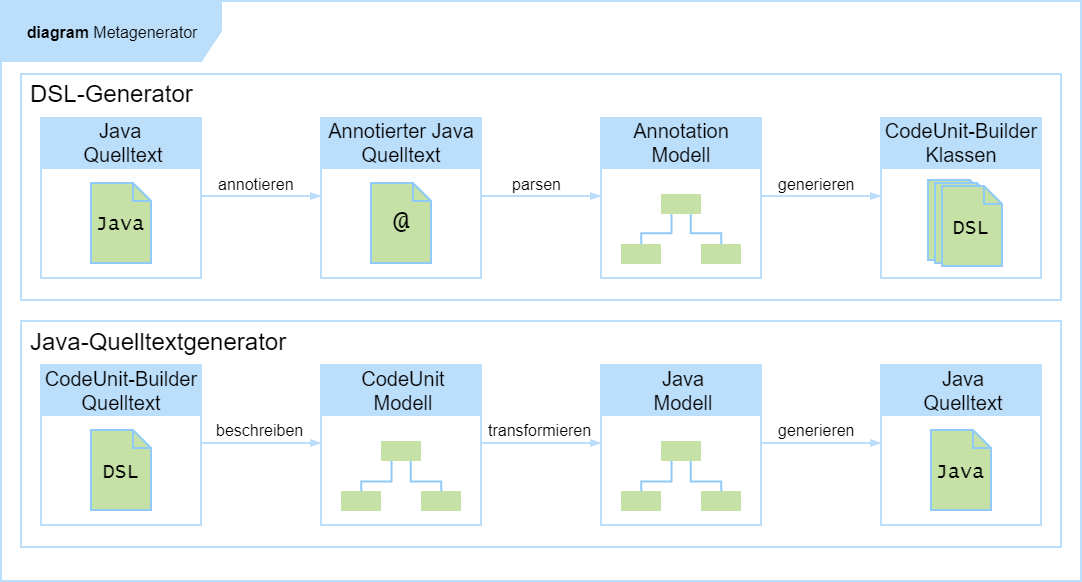
\includegraphics[width=1.0\textwidth]{bilder/metagenProzess}
	\caption{Darstellung der Prozessstruktur des Java-Metagenerators.}
	\label{fig:meta1}
\end{figure}

\section{Funktionsweise des Metagenerators}

Das Konzept der einzelnen Schritte und der hierfür verwendeten Ansätze wird im folgenden, orientiert an der obigen Prozessstruktur, detailliert erläutert.

\subsection{Von Java-Quelltext zum Annotations-Modell}

Ausgehend von einer Referenzimplementation muss diese, wie bereits in der Analyse beschrieben, mit Informationen angereichert werden um Variabilitäten zur Generierung einer DSL ausdrücken zu können.

Das Konzept sieht vor, dass Java Elemente entweder als statisches oder als variables Element markiert werden können. Da nur für variable Elemente ein Builder erzeugt wird, müssen statische Elemente stets innerhalb eines variablen Elements stehen. Das bedeutet beispielsweise, dass eine Klasse als variabel gekennzeichnet wird und dadurch einzelne Felder innerhalb der Klasse als statisch oder variabel markiert werden können. Elemente die weder als statisch noch als variabel gekennzeichnet wurden und nicht implizit zu einem übergeordneten Element gehören, werden beim parsen nicht beachtet. Ein statisches Java Element soll hierbei als vordefiniert verstanden werden, ein Beispiel hierfür wäre ein ID Feld einer Klasse.

Als Alternative zur expliziten Markierung einzelner Elemente als statisch, wäre es stattdessen denkbar gewesen alle nicht markierten Elemente als statisch zu interpretieren. Dies hätte zur Folge gehabt, dass es nicht möglich gewesen wäre Elemente der Referenzimplementation zu ignorieren. Damit wären Fälle in denen zwei gleichartige Elemente unter einer CodeUnit mit einer bestimmten Variabilität zusammengefasst werden sollen nicht ohne weiteres umsetzbar. Es sei denn es würde eine weitere Markierung eingeführt welche dafür sorgt das an Element explizit ignoriert wird. Hierunter könnte die Lesbarkeit des markierten Quelltextes leiden und für die Markierung hätte ein zusätzliches Schlüsselwort eingeführt werden müssen.

\subsubsection{Annotationen als Mittel zur Informationsanreicherung}

Im letzten Kapitel wurden drei Ansätze aufgezeigt um Java Quelltext mit zusätzlich Informationen zu hinterlegen. Diese sind die Verwendung einer externen Modelldatei mit Referenzen zum Java Quelltext, Kommentierung von Quelltext Zeilen bzw. Abschnitten mit den zusätzlichen Daten in einer speziellen Syntax oder Markierung von Codeelementen mit Annotationen.

Für dieses Konzept sind Annotationen das Mittel der Wahl. Sie kombinieren einige Vorteile der beiden anderen Ansätze. Da ein Anwender des Metagenerators den Schritt der Informationsanreicherung manuell durchführen muss, bietet ihm die Einschränkungsmöglichkeit der Anwendbarkeit von Annotationen auf bestimmte Elemente des Codes eine Hilfestellung und reduziert mögliche Fehler. Die Annotationen sind hier eine verteilte interne DSL und somit stellt jede Annotationen ein Schlüsselwort dieser internen DSL dar. Im Gegensatz zur Verwendung von Kommentaren hat ein Entwickler also rudimentäre IDE Unterstützung. 

Der Vorteil einer externen XML-Modelldatei mit entsprechender XSD, dass die Struktur klar definiert und eingeschränkt werden kann, kommt nur beim parsen der XML Daten zum tragen, bietet aber keinerlei Hilfe während ein Entwickler die Variabilitäten definiert. Zudem müsste hierfür ein System zur Referenzierung einzelner Code Zeilen eingeführt werden. Durch Annotationen ist die Zugehörigkeit zu einem bestimmten Codeelement eindeutig.

Sowohl bei der Verwendung von Kommentaren, als auch von externen Modell-Dateien müsste ein Entwickler unter Umständen ein komplett neuartiges Konzept lernen. Für Kommentare müsste eine extra Syntax verwendet werden und bei externen Modell-Dateien zum Beispiel XML. Annotationen erlauben es dem Entwickler im Java Sprachraum zu bleiben und reduzieren somit möglicherweise den zusätzlichen Lernaufwand.

\subsubsection{Parsen des annotierten Codes}

Für dieses Konzept wird der annotierte Java-Quelltext mithilfe einer externen Bibliothek geparsed. Diese Entscheidung wurde getroffen, da ein möglichst großer Teil des Java Sprachschatzes vom Metagenerator abgedeckt sein sollte. Während der Entwicklung hätte dies zur Folge, dass der Parser sukzessiv mit dem Metagenerator erweitert werden müsste, welches den Arbeitsaufwand signifikant erhöht hätte.

Die konkrete Wahl ist auf die Bibliothek JavaParser in Kombination mit dessen Erweiterung JavaSymbolSolver in der Version 0.6.3 gefallen. Beides ist unter http://javaparser.org/ zu finden und dort mit Anleitungen und Codebeispielen versehen. Das aktive GitHub-Repository mit mehreren tausend Commits weckt den Anschein, dass JavaParser ständig aktualisiert und weiterentwickelt wird. Außerdem kann der von der Bibliothek bereitgestellte AST leicht mithilfe des Visitor Patterns weiterverarbeitet werden. JavaSymbolSolver kommt zum Einsatz, da an einigen Stellen im Proof-of-Concept voll qualifizierte Datentypen benötigt werden welche aus dem normalen AST nicht ohne Zusatzaufwand gewonnen werden konnten. Genauere Informationen zur Verwendung von JavaParser und JavaSymbolSolver werden im Kapitel zur tatsächlichen Umsetzung dieses Konzepts bereitgestellt.

\subsubsection{Zweck des Annotations-Modells}

Mit dem Visitor Pattern wird der von JavaParser bereitgestellte AST untersucht. Je nach Annotation und annotiertem Java-Ausdruck wird aus diesen gewonnenen Informationen ein oder mehrere Annotations-Modelle instanziiert. Ein Instanz des Annotations Modells hält dabei immer alle Informationen zu den statischen und variablen Bestandteilen die später mit dem CodeUnit-Modell abgebildet werden, bzw. mit den generierten CodeUnit-Buildern beschrieben werden können. 

Das Annotations-Modell wurde als Zwischenschritt von AST zur konkreten DSL konzeptioniert, da dies losgelöst vom Parser im Sinne der Modularisierung ermöglicht, den aktuellen DSL Generator durch eine andere Komponente zu ersetzen. Durch das Annotations-Modell liegen hierfür bereits alle notwendigen Informationen abstrahiert vor und müssen nicht erneut aus dem AST ausgelesen werden.

\subsection{Das CodeUnit-Modell}

Ein wichtiger Teil dieses Konzepts ist das CodeUnit-Modell. Instanzen dieses Modells werden von den generierten CodeUnit-Buildern beschrieben und somit ist es das Metamodell für die vom Metagenerator erzeugte DSL. Mit einer spezifischen CodeUnit-Annotation und unter Angabe einer Benennung, kann ein Java Element so markiert werden, dass hieraus ein Annotations-Modell geparsed wird. Aus den so entstandenen Annotations-Modellen wird in einem nachgelagerten Schritt die interne DSL erzeugt.

\subsubsection{Aufbau des Modells}

Das CodeUnit Modell setzt sich aus einer Struktur mehrerer CodeUnits zusammen, diese sind dabei hierarchisch geordnet. An jede CodeUnit können SubCodeUnits angehängt werden, aber es gibt stets genau eine CodeUnit welche das Wurzelelement des darunterliegenden Baumes ist. Der Aufbau jedes CodeUnit-Modells ist gleich, einzelne CodeUnits unterscheiden sich nur in ihren konkreten Parametern.

Diese Struktur wurde gewählt, da Quelltext sich in einer solchen hierarchischen Folge gut ausdrücken lässt. Bei Java gibt es beispielsweise Klassen welche Felder und Methoden haben, dies wird im CodeUnit-Modell als eine CodeUnit für die Klasse mit SubCodeUnits für Felder und Methoden abgebildet. Die CodeUnit für eine Methode könnte wiederum SubCodeUnits für Parameter und den Methoden Körper haben. Dieser beschriebene Zusammenhang ist beispielhaft in Abbildung ~\ref{fig:cu1} dargestellt.

\begin{figure}[htbp]
	\centering
	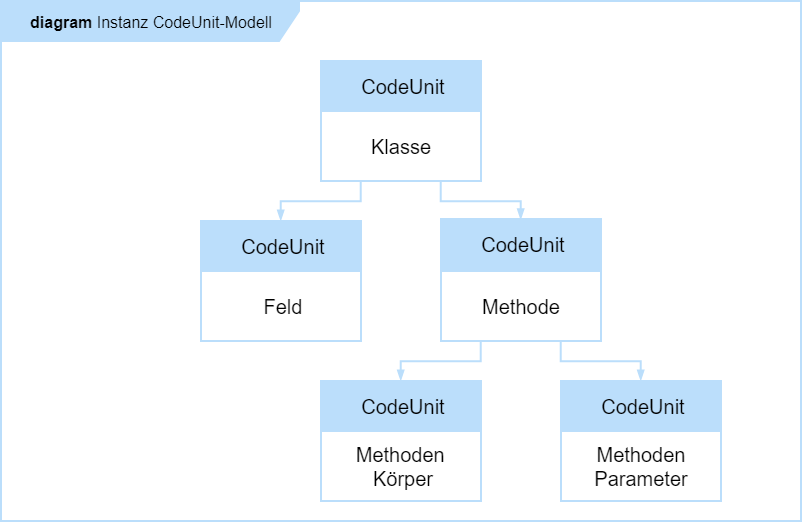
\includegraphics[width=1.0\textwidth]{bilder/cuModelBsp}
	\caption{Beispielhafte Darstellung der Struktur eines CodeUnit-Modells.}
	\label{fig:cu1}
\end{figure}

\subsubsection{Spezialisierung durch ein Typ-Feld}

Um später eine konkrete Instanz des CodeUnit Modells zu einer Java-Modell Instanz transformieren zu können, müssen wichtige semantische Informationen vorliegen. Eine hiervon ist, welche Art von Java Element mit dieser CodeUnit abgebildet wird. Jede CodeUnit hat einen CodeUnit-Typen an welchem der Transformator später erkennt auf welche Weise die spezifische CodeUnit in das Java-Modell transformiert werden muss.

Für das Konzept wurde hierfür kein objektorientierter Ansatz gewählt, bei welchem für jeden CodeUnit Typ eine eigene CodeUnit Klasse implementiert werden würde. Das Argument gegen spezielle CodeUnit Klassen ist, dass die CodeUnit Klasse hier ein Datenmodell darstellt welches kein eigenes Verhalten hat. Somit wäre jede abgeleitete Klasse von CodeUnit nur eine, durch ihre Benennung, semantische Erweiterung, aber ansonsten funktionslos. Zudem reduziert der gewählte Ansatz den Aufwand bei der Erweiterung der CodeUnit-Struktur um neue CodeUnit-Typen.

Als Ausnahme könnte man CodeUnits welche mit Buildern beschreibbar sind zählen. Da mit einem Builder für eine Klassen-CodeUnit unter Umständen eine Feld-CodeUnit als SubCodeUnit angehängt wird, hätte man hier durch die Einführung von eigenen Datentypen die Möglichkeit einzuschränken welche Typen von CodeUnits als SubCodeUnits verwendbar sind. Diese Klassen würden dann nur für diese Eigenschaft existieren keine weiteren Funktionen haben.

\subsubsection{Parametrisierung durch generische Datenstruktur}

Wie beschrieben wird jeder CodeUnit-Typ in seiner Struktur gleich dargestellt. Konfigurationsdaten zu einer CodeUnit werden in einer allgemein gehaltenen Datenstruktur gespeichert. Dies ermöglicht es jede Art von Datum in einer CodeUnit zu hinterlegen. Mögliche Daten wären hier zum Beispiel der Identifier einer Klasse oder der Java-Datentyp eines Feldes.

Durch diesen Ansatz, in Kombination mit dem Typ der CodeUnit, kann das CodeUnit-Modell sehr einfach erweitert oder abgeändert werden ohne in dessen zugrunde liegende Struktur eingreifen zu müssen. Änderungen an den Schnittstellen für Transformator und DSLs werden vermieden.

Beispiele für solche Parameter wären der Identifier Parameter welchem als Datum eine Zeichenkette zugeordnet ist und der Modifier Parameter zu welchem ein Array aus Java Modell Feuer Schlüsselwörtern angegeben wird. Ein solches Datum kann auch zur Markierung einer Eigenschaft der zugehörigen CodeUnit verwendet werden, in dem, unter einer geeigneten Parameter Benennung, zum Beispiel ein Bool'scher Wert hinterlegt wird.

\subsection{Generierung von Buildern als interne DSL aus dem Annotations-Modell}

Grundsätzlich wäre, wie in der Analyse beschrieben,  für dieses Konzept sowohl eine externe DSL als auch eine interne DSL denkbar gewesen. Der für eine externe DSL notwendige Mehraufwand bzw. die Toolbindung bei Verwendung einer Language Workbench waren hier jedoch ausschlaggebend für die Entscheidung zur internen DSL. Außerdem gilt, genau wie bei dem Argument für Annotationen, dass bei der Verwendung einer internen DSL auf Java Basis die Anwendung potentiell einfacher ausfällt. Durch das Annotations-Modell wäre es jedoch denkbar aus diesem eine externe DSL zu generieren.

Die konkrete Umsetzung einer internen DSL bietet mehrere Ansätze. Zum einen könnte man hier auf Sequenzen aus Funktionen zurückgreifen, hat damit aber keine Kontrolle darüber in welcher Reihenfolge der Entwickler die verschiedenen Statements aufruft. Unter Verwendung eines Kontextobjekts wäre es lediglich möglich bei einer unerlaubten Sequenz Fehler auszugeben oder Ausnahmen zu werfen\,\cite[S. 351ff.]{fowler2010}. Alternativ hierzu könnte ein Builder Pattern mit Method Chaining zum Einsatz kommen. Dies würde große Kontrolle darüber ermöglichen welche Statements in welcher Reihenfolge ausführbar sind\,\cite[S. 343ff.]{fowler2010}. Eine weitere Möglichkeit zur Implementation einer internen DSL wäre die Verwendung von geschachtelten Methoden. Hierdurch kann ebenso stark kontrolliert werden in welcher Reihenfolge Methoden einer Sequenz anwendbar sind. Da die verschachtelten Funktionen von innen nach außen evaluiert werden, muss man besondere Rücksicht hierauf nehmen\,\cite[S. 357ff.]{fowler2010}.

Für dieses Konzept wurde, wie schon mehrfach erwähnt, auf ein Builder Pattern mit Method Chaining zurückgegriffen. Hauptargument hierfür war die mögliche Kontrolle über die Reihenfolge der ausführbaren Statements. Da sowohl verschachtelte Methoden als auch Builder ähnliche Vorteile haben wurde zwischen diesen auf Basis persönlicher Präferenz entschieden. Wird an eine CodeUnit eine SubCodeUnit angehängt, ist diese ein Parameter der aufgerufenen Builder Methode und somit handelt es sich hier im kleinen Rahmen um eine Verschachtelung.

\subsubsection{Erzeugte Builder als Schlüsselwörter der internen DSL}

Aus jedem Annotations Modell wird ein konkreter Builder erzeugt. Jedes dieser Modelle ist ursprünglich durch eine spezifische CodeUnit Annotationen entstanden und hat hierdurch auch eine Benennung erhalten. Die Idee dahinter ist, dass es möglich sein soll, bestimmte Attribute eines Java Elements nicht variabel zu machen und somit eine gewisse Form der Abstraktion zu bieten. Mit einer aussagekräftigen Benennung der beschreibbaren CodeUnit, kann hieraus auch ein eindeutig identifizierbarer Builder generiert werden.

Man nehme beispielsweise den Fall, dass ein Java Feld als CodeUnit mit einem Builder beschreibbar sein soll. Unter Verwendung entsprechender Annotationen könnte diese CodeUnit immer als öffentlich mit variablem Datentyp markiert werden. Hinzu käme eine sprechende Benennung wie zum Beispiel PublicVar. Hieraus könnte dann ein PublicVarBuilder generiert werden, welcher immer eine öffentliches Feld erzeugt und die Fähigkeit hat dessen Datentyp zu setzen.

Werden auf diese Weise mehrere Builder zur Beschreibung unterschiedlich konfigurierter CodeUnits mit unterschiedlichem CodeUnit Typ erzeugt, so entwickelt sich dadurch ein DSL Sprachraum mit konkreter Semantik. Die einzelnen Builder könnte man in diesem Sprachraum als Schlüsselwörter der internen DSL betrachten.

\subsubsection{Komposition der Builder aus benötigten Builder-Methoden}

Abhängig davon welcher CodeUnit Typ von einem konkreten Builder beschrieben werden kann und welche Variabilitäten in Form von Annotationen in der Referenzimplementation definiert wurden, hat ein CodeUnit Builder unterschiedliche Methoden. 

Ein Builder zur Beschreibung des im letzten Abschnitt gegebenen Beispiels eines öffentlichen Feldes mit variablem Datentyp, benötigt beispielsweise keine Methode zum setzen eines Parameters für den Java-Modifier. Jedoch benötigt jeder Builder eine Methode zum Starten der Method Chain und eine um die Kette abzuschließen.

Der Ansatz hierfür ist Komponenten basiert. Die unterschiedlichen Methoden die ein konkreter Builder haben kann werden diesem Komponentenweise während der Erzeugung hinzugefügt. Dieses Konzept wurde gewählt, da die Alternative hierfür wäre, dass jeder Builder genau die gleichen Methoden implementiert. Hierbei müsste, um das Setzen bestimmter Werte zu verbieten, spezielles Error Handling betrieben werden. Der komponentenbasierte Ansatz schränkt die konkrete Syntax der internen DSL weiter ein und bietet somit dem Anwender eine Hilfestellung bei der Formulierung von Ausdrücken.

\subsubsection{Übertragung vorgegebener Informationen in einen Builder}

Einige der in der Referenzimplementation vorliegenden Daten müssen als solches in den am Ende der Kette generierten Java Quelltext übertragen werden. Hierunter fallen alle unveränderlichen Parameter eines als CodeUnit annotierten Java Elements die nicht durch den Typen oder den Kontext der CodeUnit impliziert werden und jedes als statisch annotierte Java Element.

Hierfür sieht dieses Konzept vor bereits beim parsen des annotierten Java Quelltextes eine Ursprungs-CodeUnit zu jedem Annotations Modell zu erzeugen. Diese CodeUnit dient dann dem aus dem Annotations Modell generierten Builder als Ausgangspunkt bei der Beschreibung einer konkreten CodeUnit.

Ein alternativer Ansatz wäre gewesen, eine zusätzliche Datenstruktur zum Halten dieser Informationen zu verwenden. Im Aufbau würde dieses zusätzliche Modell jedoch sehr dem der CodeUnit ähneln, da gleichartige Daten hinterlegt werden würden. Daher kann auch direkt und ohne Mehraufwand das bereits bestehende CodeUnit Modell verwendet werden.

\subsubsection{Verwendung von Plattform Code zur Generierung von vordefinierten CodeUnits und Fehlermanagement}

Bei der Anwendung eines Builders kann es vorkommen, dass vordefinierte CodeUnits in das vom Builder beschriebene CodeUnit Modell eingefügt werden müssen. Als konkretes Beispiel dienen hier Getter und Setter Methoden für ein Feld. Ein solches könnte mit einer CodeUnit und einer HasGetter Annotation versehen werden. Dies würde semantisch bedeuten, dass immer, wenn diese Feld-CodeUnit mit einem Builder beschrieben und an eine Klassen-CodeUnit angehängt wird, ebenfalls eine auf dieses Feld zugreifende Getter-CodeUnit erzeugt werden soll.

Auf solche vordefinierten CodeUnits kann aus vielen Buildern zugegriffen werden. Sie unterscheiden sich teilweise gar nicht oder nur in einzelnen Parametern, wie zum Beispiel bei einem Getter dem Feldnamen. Deswegen kommt hier Plattform Code zum erzeugen dieser CodeUnits zum Einsatz. Dieser bildet folglich eine Abhängigkeit zur Verwendung von generierten Buildern.

Plattform Code wird ebenfalls verwendet um eine CodeUnit zu prüfen bevor ihr Builder abgeschlossen wird.

\subsubsection{Auflösung von Referenzen in vordefinierten CodeUnits als nachgelagerter Verarbeitungsschritt}

Es ist möglich, dass ein als statisch annotiertes Feld den selben Datentyp hat wie dessen zugehörige Klasse. Eine solche Referenz auf den eigenen Typen kommt zum Beispiel beim Instanz Feld eines Singleton vor. Wird jetzt eine CodeUnit basierend auf einer solchen Situation beschrieben, sollte auch die entsprechende Referenz auf den angegebenen neuen Identifier der zugehörigen Klasse verweisen.

Der früheste Zeitpunkt an dem bei der Verwendung eines Builders für eine Klassen-CodeUnit klar ist welche SubCodeUnits diese hat, ist wenn die Method Chain explizit beendet wird. Bevor die endgültige CodeUnit zurückgegeben wird ist ein letzter Verarbeitungsschritt vorgesehen. 

Jede SubCodeUnit der Klasse wird nach Referenzen auf den ursprünglichen Datentyp aus der Referenzimplementation durchsucht und an dessen Stelle tritt durch Textersetzung der neue, tatsächliche Identifier der erzeugten Klassen-CodeUnit. Die Information hierzu wird, wenn benötigt, bei der Erzeugung des Annotations Modells in der Ursprungs-CodeUnit als Parameter hinterlegt.

Der aktuelle Proof of Concept ersetzt in diesem Nachbearbeitungsschritt nur Referenzen auf die Ursprungsklasse und erzeugt Standard CodeUnits, wie zum Beispiel Getter und Setter. Erweiterungen dieser nachgelagerten Phase sind jedoch durchaus denkbar.

\subsection{Erzeugung von Java Code aus einem befüllten CodeUnit-Modell}

In diesem Konzept wird aus dem instanziierten CodeUnit Modell nicht direkt Java Quelltext erzeugt. Stattdessen wird das CodeUnit Modell in ein allgemeines Java Modell überführt und dieses wird als Eingabe für ein allgemeinen Java Code Generator verwendet. Diese zusätzliche Schicht wurde in den Generator eingebaut um, wie auch bereits die Entscheidung zum Annotations Modell begründet wurde, die Modularität des gesamten Konzeptes zu erhöhen. Denn hiervon Ausgehend ist es jetzt möglich eine CodeUnit auch in andere Sprachen  bzw. Modelle zu transformieren. Liegt bereits ein Code Generator für eine Sprache vor, so könnte dieser wiederverwendet werden in dem man das CodeUnit Modell zu einem für diesen Generator verständlichen Modell überführt.

\subsubsection{Transformation des CodeUnit-Modells zum Java-Modell}

Für die Umwandlung des CodeUnit Modells zum Java Modell wird, ausgehend vom Wurzelelement, eine CodeUnit anhand von Transformationsregeln iterativ umgewandelt. Die Wahl der Transformationsregel basiert auf dem CodeUnit Typen.

Das verwendete Java Modell stellt nur eine Teilmenge des Java Metamodells dar und bildet nur Java sprach Features ab welche mit den generierten DSLs in einer CodeUnit beschreibbar sind. Mit jeder Funktionserweiterung des Proof-of-Concept, geht auch eine Erweiterung des verwendeten Java Modells einher. Das Java Modell soll jetzt keine abstrakte Darstellung von Quelltext mehr sein sondern gezielt und so genau wie möglich die Struktur von Java Quelltext abbilden.

\subsubsection{Erzeugung von Quelldateien}

Zur Generierung von Java Quelltext wird bei diesem Konzept Transformer Generation verwendet. Der Vorteil Template basierter Quelltexterzeugung des reduzierten Aufwands, wenn sich viele Teile des Generats wiederholen, kann bei der vorliegenden Problemstellung nicht ausgenutzt werden. Die vom Metagenerator erzeugten Java Quelltext Dateien können in ihrem Inhalt praktisch vollständig voneinander abweichen.

Zur konkreten Java Quelltexterzeugung wurde im Proof of Concept auf eine externe Bibliothek zugegriffen. Zum Einsatz kommt hier JavaPoet in der Version 1.9.0 für welches unter~\cite{javapoet2017} eine Informationsseite hinterlegt ist. JavaPoet wurde gewählt da es eine, auf Method Chaining basierende, gut verständliche API zum Erstellen spezifischer Java Quelltextteile bereitstellt. Zudem wird JavaPoet regelmäßig aktualisiert.

\chapter{Lösung: Spectrum (Proof of Concept)}

Parallel zur Konzeptionierung und um schlussendlich das Konzept auch grundsätzlich zu validieren, wurde für diese Arbeit ein Proof of Conzept umgesetzt. Der hierbei entstandene Metagenerator hat die Bezeichnung Spectrum.

Im folgenden Kapitel werden zuerst die im letzten Kapitel bereits erwähnten, in Spectrum eingesetzten externen Bibliotheken mit kurzen Anwendungsbeispielen vorgestellt. Gefolgt wird dies von einer allgemein Architekturübersicht über die Komponenten von Spectrum, welche dann in den darauf folgenden Abschnitten genau erläutert werden. Neben einer Beschreibung der Funktionalität der Komponente wird auch deren Umsetzung näher betrachtet. Wichtige Stellen der Implementation und bei Bedarf die Anwendung einer Komponente werden anhand von Codebeispielen detaillierter dargestellt.

\section{Eingesetzte externe Bibliotheken}

Wie bereits im Konzept erläutert, wurde sowohl zum einlesen der Referenzimplementation als auch zur späteren Java Quelltexterzeugung auf externen Bibliotheken zugegriffen. Um diese Abhängigkeiten leicht handhaben zu können, wurde für die Implementation Apache Maven verwendet, welches unter https://maven.apache.org/ bezogen werden kann. Moderne integrierte Entwicklungsumgebungen, wie beispielsweise IntelliJ, unterstützen Maven ohne zusätzliche Installationsschritte.

\subsection{JavaParser mit JavaSymbolSolver}

Die Entwickler von JavaParser und JavaSymbolSolver beschreiben ihre Bibliothek als Möglichkeit zur Interaktion mit Java Quelltext in Form einer Objekt Repräsentation. Mit Objekt Repräsentation ist hier ein AST gemeint. Zusätzlich soll mit Unterstützung des Visitor Patterns ein praktischer Mechanismus zur Traversierung des AST zur Verfügung gestellt werden. Zusätzlich könnte mit dem Java Parser der AST manipuliert und wieder in eine Datei überführt werden\,\cite[S. 1]{javaparser2017}. Dieses Feature wird in Spectrum jedoch nicht verwendet.

\subsubsection{Anwendung}

\begin{lstlisting}[label=lst:jpVisit,
language=java,
firstnumber=1,
caption=Beispielhafte Initialisierung und Verwendung des JavaParsers und des JavaSymbolSolvers]
class ExampleParser {
	public void handle(File file) {
		//parse sourcecode file
		CompilationUnit cu = JavaParser.parse(file);
		
		//inject TypeSolver
		TypeSolver ts = new ReflectionTypeSolver();
		JavaSymbolSolver jss = new JavaSymbolSolver(ts);
		jss.inject(cu);
		
		//visit with VariableVisitor
		new VariableVisitor().visit(cu, null);
	}
}

private static class VariableVisitor extends VoidVisitorAdapter<Void> {
	@Override
	public void visit(VariableDeclarator declarator, Void arg) {
		//resolve declarator and get qualified identifier
		String qualifiedVariableName = declarator
										.resolve()
										.asReferenceType()
										.getQualifiedName();
		
		//do something with qualifiedVariableName;
	}
}
\end{lstlisting}

Um mit JavaParser arbeiten zu können, wird zuerst eine vorhandenen Java Quelltext Datei geparsed. Das Endprodukt des Parsing Prozesses heißt bei JavaParser CompilationUnit, hierunter sind in hierarchische Ordnung alle Knotenpunkte des AST gesammelt. Zur Traversierung der CompilationUnit können Visitor implementiert werden. Diese ermöglichen es den Baum gezielt nach Knotenpunkten mit bestimmten Eigenschaften zu durchlaufen. Hierfür wird eine Klasse mit einer Visit-Methode implementiert welche einen von JavaParser zur Verfügung gestellten VisitorAdapter erweitert. Der Typ-Parameter des erweiterten VisitorAdapters ist in der Signatur der Visit-Methode wiederzufinden. Über den zweiten Parameter dieser Methode kann, wenn ein Typ-Parameter angegeben wird, ein Kontextobjekt übergeben werden.

Um mit JavaSymbolSolver Symbole auflösen zu können um beispielsweise auf den vollständig qualifizierenden Namen einer Klasse zuzugreifen, muss ein JavaSymbolSolver Objekt instanziiert werden. Dafür wird eine Instanz eines TypeSolvers benötigt. Diese werden in JavaParser: Visited genauer erklärt\,\cite[S. 39ff.]{javaparser2017}. 

Der genaue Typ des TypeSolvers steuert wo genau nach Typ Referenzen gesucht wird. Ein JarTypeSolver sucht beispielsweise nur innerhalb einer bestimmten JAR-Datei und ein ReflectionTypeSolver sucht, wie der Name schon sagt, nach Klassen Referenzen via Reflection. Das Listing ~\ref{lst:jpVisit} zeigt die in diesem Abschnitt erläuterten Features von JavaParser und JavaSymbolSolver in einer beispielhaften Anwendung.

\subsubsection{Installation mit Maven}

\begin{lstlisting}[label=lst:jpmaven,
language=HTML,
firstnumber=1,
caption=XML-Code zum Einbinden von JavaParser und JavaSymbolSolver als Maven-Dependency.]
<dependency>
	<groupId>com.github.javaparser</groupId>
	<artifactId>java-symbol-solver-core</artifactId>
	<version>0.6.3</version>
</dependency>
\end{lstlisting}

Bei der Verwendung von JavaParser und JavaSymbolSolver in Kombination, muss lediglich die Abhängigkeit zu JavaSymbolSolver in die pom.xml eingetragen werden. JavaSymbolSolver beinhaltet automatisch die aktuellste kompatible JavaParser Version. Der XML-Code zum Einbinden des JavaSymbolSolver als Maven-Dependency wird in Listing ~\ref{lst:jpmaven} dargestellt.

\subsection{JavaPoet}

JavaParser hätte zwar grundsätzlich die Möglichkeit zur Erzeugung von Java Quelltext Dateien geboten, im Gegensatz zu JavaParser hat JavaPoet jedoch zusätzlich eine gut lesbare API zur Beschreibung des zu erzeugenden Quelltextes.

\subsubsection{Anwendung}

\begin{lstlisting}[label=lst:jpoet,
language=java,
firstnumber=1,
caption={Java-Quelltext zur Erzeugung eines \glqq Hallo, Welt!\grqq -Beispiels, angelehnt an das \glqq Hello, JavaPoet!\grqq{} Beispiel in der README.md von\,\cite{javapoet2017}.}]
class HelloWorldGenerator {
	public String generateHelloWorld() {
		MethodSpec mainMethodSpec = MethodSpec.methodBuilder("main")
		.addModifiers(Modifier.PUBLIC, Modifier.STATIC)
		.addParameter(String[].class, "args")
		.addStatement("$T.out.println($S)", System.class, "Hello, World!")
		.returns(void.class)
		.build();
		
		TypeSpec exampleTypeSpec = TypeSpec.classBuilder("Example")
		.addModifiers(Modifier.PUBLIC, Modifier.FINAL)
		.addMethod(mainMethodSpec)
		.build();
		
		JavaFile javaFile = JavaFile.builder("example.package.name", exampleTypeSpec)
		.build();
		
		String javaCodeString = javaFile.toString();
	}
}

//above generateHelloWorld()-Method returns the following String
package example.package.name;

public final class Example {
	public static void main(String[] args) {
		System.out.println("Hello, World!");
	}
}

\end{lstlisting}

Auf Basis von mehreren Buildern werden die verschiedenen Teile einer Java Klasse zuerst modelliert, um dieses Modell dann später als Java Quelltext auszudrücken. Die Ausnahme bilden hier Methoden Körper, diese werden bei JavaPoet in Form von Strings verwaltet.

Soll in einzelnen Ausdrücken ein bestimmtes Datum in einer Zeichenkette verwendet werden, müssen diese nicht mit einzelnen Operatoren konkateniert werden. Um die API lesbarer zu gestalten wurde in JavaPoet eine, an Javas String.format() angelehnte, Kurzschreibweise implementiert. Hierdurch können in einer Zeichenkette Platzhalter verwendet werden deren Inhalt zusätzlich als Parameter an die entsprechende Funktion übergeben wird. Dies ist vor allem hilfreich wenn diese Parameter dynamisch sind. Hierunter fällt zum Beispiel der Platzhalter \$L für Literale welche direkt und unverändert in den einbettenden String übernommen werden. Ein weiterer Platzhalter ist \$T, dieser kann verwendet werden um eine Referenz auf einem bestimmten Datentypen zu hinterlegen. Es gibt noch einige weitere dieser Platzhalter, diese werden gut, zusammen mit weiteren Features, in der JavaPoet README.md des zugehörigen GitHub Repositories erklärt\,\cite{javapoet2017}. Listing~\ref{lst:jpoet} zeigt die Verwendung von Java Poet anhand eines einfachen Beispiels.

\subsubsection{Installation mit Maven}

\begin{lstlisting}[label=lst:jpoetmaven,
language=HTML,
firstnumber=1,
caption=XML-Code zum Einbinden von JavaPoet als Maven-Dependency.]
<dependency>
	<groupId>com.squareup</groupId>
	<artifactId>javapoet</artifactId>
	<version>1.9.0</version>
</dependency>
\end{lstlisting}

Zur Einrichtung der Maven-Dependency von JavaPoet kann der in Listing~\ref{lst:jpoetmaven} dargestellte XML-Code verwendet werden. 

\section{Architekturübersicht}

\begin{figure}[htbp]
	\centering
	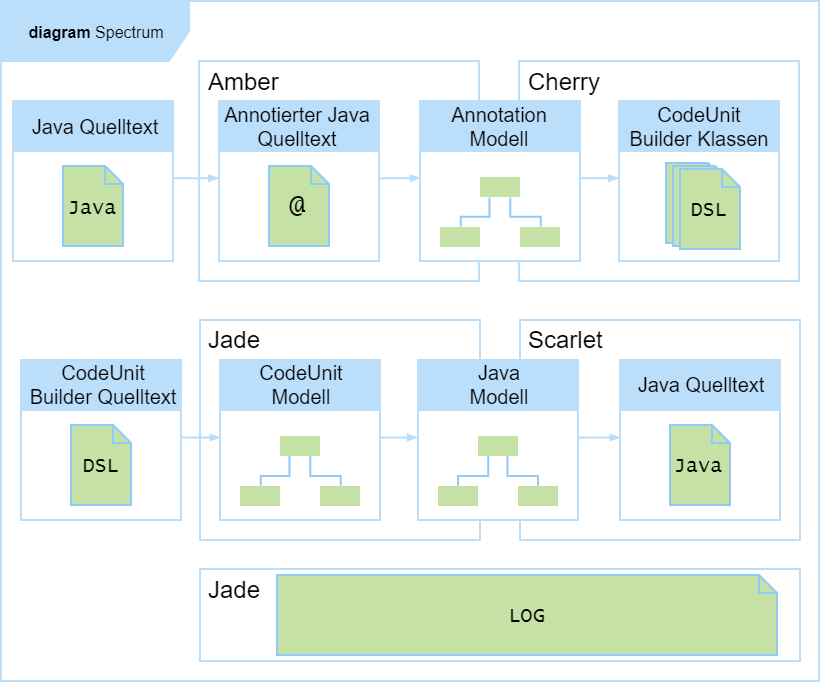
\includegraphics[width=1.0\textwidth]{bilder/spectrumPackages}
	\caption{Darstellung der Komponenten von Spectrum.}
	\label{fig:spectrumPackages}
\end{figure}

Die allgemeine Architektur von Spectrum orientiert sich an der Funktionalität einzelner Komponenten. Insgesamt besteht Spectrum aus fünf Java Packages: Amber, Cherry, Jade, Scarlet und Violet. Jede dieser Komponenten hat eine klare Aufgabe im Metagenerator Gesamtprozess. Die Grafik~\ref{fig:spectrumPackages} zur Architektur von Spectrum, welche sich an der Abbildung~\ref{fig:meta1} aus dem Konzept Kapitel orientiert, zeigt unter anderem die im Prozess entstehenden Artefakte und welche Komponenten jeweils mit diesen in Berührung kommen. Die genaue Aufgabe und Implementation der Bestandteile von Spectrum werden in den folgenden Abschnitten erläutert.

\begin{figure}[htbp]
	\centering
	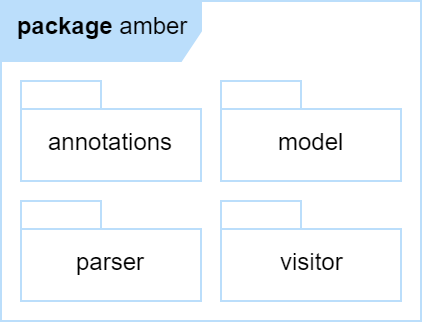
\includegraphics[width=0.5\textwidth]{bilder/amber}
	\caption{Darstellung der Unter-Packages im amber Package.}
	\label{fig:amberPackages}
\end{figure}

\subsection{Amber}

Die Bereitstellung der Annotationen zur Informationsanreicherung der Referenzimplementation und die Überführung des annotierten Quelltextes in das Annotations Modell sind die Aufgaben von Amber. Hierfür ist Amber in vier Packages unterteilt. Diese sind jeweils sprechend nach ihrer Funktion benannt. Abbildung~\ref{fig:amberPackages} stellt die Packages grafisch dar.

\subsubsection{Implementierte Annotationen}

Die Annotationen bilden die Schlüsselwörter der verteilten DSL zur Informationsanreicherung einer Referenzimplementation. In der aktuellen Version des Proof of Concept können Klassen, Felder, Methoden und Konstruktoren annotiert werden. Ist eines davon als CodeUnit markiert und als Annotations Parameter ein String übergeben, so wird hieraus ein Annotations Modell geparsed. Cherry erzeugt dann aus jeder Instanz des Annotations Modells einen Builder. Als FixedCodeUnit annotierte Elemente werden in die Ursprung-CodeUnit des logisch darüber liegenden Annotations Modells übernommen.

Alle zur Informationsanreicherung verfügbaren Annotationen sind im Package annotations zu finden. Grundsätzlich gibt es für diese Annotationen mehrere Einschränkungen. Durch eine Target-Annotationen wird gesteuert an welche Teile des Java Quelltextes die Annotationen überhaupt angebracht werden darf, diese Einschränkung wird also normalerweise von der verwendeten IDE erzwungen. Abbildung~\ref{fig:tblAnnoTrgt} zeigt auf wo jeweiligen Annotationen stehen dürfen. Es existieren noch weitere, nicht erzwungene Restriktionen welche durch den Parsing Prozess eingehalten werden. Allgemein sind die einzigen beiden Annotationen welche eigenständig verwendet werden dürfen die CodeUnit und FixedCodeUnit Annotationen. Alle anderen Annotationen können nur in Kombination mit diesen beiden stehen. Einige der Einschränkungen beruhen auf deren semantischen Zusammenhang, denn beispielsweise eine HasGetter Annotation macht nur an einem Feld Sinn. Andere Limitierungen sind auf den aktuellen Entwicklungsstand zurückzuführen.

\begin{figure}[htbp]
	\centering
	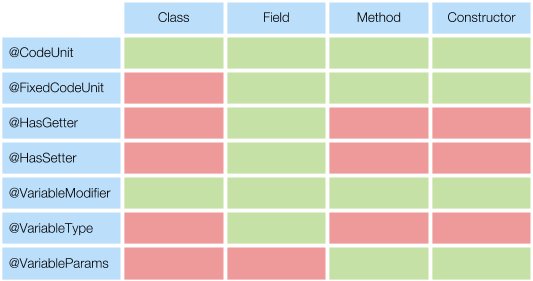
\includegraphics[width=0.75\textwidth]{bilder/tblAnnoTrgt}
	\caption{Darstellung der legalen Ziele für Amber Annotationen.}
	\label{fig:tblAnnoTrgt}
\end{figure}

\subsubsection{Bedeutung und Limitationen der Annotationen und deren Auswirkung auf die erzeugten Builder}

In den nachfolgenden Absätzen werden die unterschiedlichen Annotations Ziele und die Wirkung einer bestimmten Annotationen hierauf zusammengefasst. Zudem wird auf, durch den aktuellen Stand der Implementation bedingte, Einschränkungen eingegangen.

\begin{lstlisting}[label=lst:classanno,
language=java,
firstnumber=1,
caption=Darstellung der Annotationsmöglichkeiten an einer Klasse.]
@CodeUnit("ExampleClass") @VariableModifier
public class ExampleRef {
//...
}
\end{lstlisting}

Listing~\ref{lst:classanno} zeigt die Annotationsmöglichkeiten an einer Klasse. Eine Klasse kann nur als CodeUnit und optional mit VariableModifier markiert werden. Hierdurch wird ein Builder für die Klasse mit dem in der CodeUnit übergebenen Namen erzeugt. Eine Klasse darf dabei jede Kombination von Java-Modifiern haben. Liegt eine VariableModifier Annotation vor, müssen gewünschte Modifier explizit mit dem später erzeugten Builder gesetzt werden, an der Referenzklasse vorhandene Modifier werden standardmäßig ignoriert. Es werden keine weiteren Informationen der Klasse, zum Beispiel Interfaces und generische Typparameter, berücksichtigt. Diese müssten jedoch lediglich im Nachgang implementiert werden. Details zum Erweiterungsprozess werden im Anschluss an dieses Kapitel beschrieben.

\begin{lstlisting}[label=lst:fieldanno,
language=java,
firstnumber=1,
caption=Darstellung der Annotationsmöglichkeiten an einer Klasse.]
@CodeUnit("ExampleClass")
public class ExampleRef {
	@FixedCodeUnit @HasGetter @HasSetter
	private int id;

	@FixedCodeUnit
	protected static float f;

	@CodeUnit("PublicString") @HasGetter @HasSetter
	public String s;

	@CodeUnit("Variable") @VariableModifier @VariableType
	Object o;
}
\end{lstlisting}

Das Listing~\ref{lst:fieldanno} zeigt die Annotationsmöglichkeiten an einem Feld, fast jede der Annotationen, außer VariableParams, kann hier angebracht werden. Genau wie bei einer Klasse wird aus einem Feld welches als CodeUnit annotiert ist ein Annotations Modell gebildet, ist es als FixedCodeUnit markiert, wird das Feld in die Ursprungs-CodeUnit des zugehörigen Klassen Annotations Modells übernommen. Bei einer Annotation mit HasGetter oder HasSetter in Kombination mit FixedCodeUnit wird automatisch zum Feld noch ein Getter bzw. Setter erzeugt. Werden die beiden Annotationen zusammen mit CodeUnit verwendet, so wird jedes Mal wenn der für die CodeUnit generierte Builder genutzt wird auch ein, dem beschriebenen Feld entsprechender, Getter bzw. Setter generiert. 

Wird für das Feld ein VariableModifier oder ein variabler Typ annotiert, so verhält sich das wie die VariableType Annotation an einer Klasse: Vorhandene Daten werden ignoriert, wird eine Variabilität annotiert, müssen Werte hierfür später explizit gesetzt werden. Wurde ein variabler Datentyp nicht im Builder gesetzt, so wird bei der abschließenden Prüfung der CodeUnit ein Fehler ausgegeben und als Standardwert der Datentyp Object benutzt.

Bezüglich der Annotation von Feldern gibt es noch nicht implementierte Features. Werden in einer Zeile mehrere Felder in der Form "int a, b, c;" deklariert, wird nur das erste dieser Felder beachtet. Genauso wird eine Initialisierung bei Deklaration eines Feldes im aktuellen Proof of Concept ignoriert. Wird ein Feld als Array deklariert, wird die Deklaration als einfaches nicht-Array Feld interpretiert.

\begin{lstlisting}[label=lst:constrmethoanno,
language=java,
firstnumber=1,
caption=Darstellung der Annotationsmöglichkeiten von Konstruktoren und Methoden.]
@CodeUnit("ExampleClass")
public class ExampleRef {
	@FixedCodeUnit
	private ExampleRef() {
		//...
	}
	
	@CodeUnit("Constructor") @VariableModifier @VariableParams
	public ExampleRef(int i) {
		//...
	}
	
	@FixedCodeUnit
	public static void ExampleStaticMethod() {
		//...
	}
	
	@CodeUnit("Method") @VariableModifier @VariableParams
	void ExampleMethod() {
		//..
	}
}
\end{lstlisting}

Methoden und Konstruktoren können beide als CodeUnit oder FixedCodeUnit markiert werden. Bei einer Annotation als FixedCodeUnit wird die Methode oder der Konstruktor, genau wie bei einem Feld, in die Default-CodeUnit des Annotations Modells der übergeordneten Klasse übernommen. Entsprechend wird bei der Verwendung der CodeUnit Annotation ein Annotations Modell für die Methode oder den Konstruktor gebildet. Der Körper der Methode oder des Konstruktors muss beim Bauen immer gesetzt werden, ansonsten wird ein leerer Standard-Körper verwendet. Der Rückgabewert kann ebenso nicht als Variabilität annotiert werden, da dieser als standardmäßig variabel angesehen wird. Als Defaultwert wird hier, bei fehlender Angabe, void angenommen. Listing~\ref{lst:constrmethoanno} zeigt die unterschiedlichen Annotations Möglichkeiten für Methoden und Konstruktoren auf.

Da vor dem parsen der Referenzimplementation keine Prüfung der Annotationen durchgeführt wird, sind Kombinationen wie ein static Feld mit einer HasGetter Annotation möglich. In der aktuellen Version wird in diesem Fall ein Getter erzeugt welcher auf eine nicht vorhandene Instanz Variable verweist. Es gibt mehrere solcher potentieller Fehlerquellen. Es macht jedoch keinen Sinn diese Fehler an andere späteren Stelle des Erzeugungsprozesses zu handhaben. Wenn dann müsste für die verteilte interne DSL aus Annotationen im Vorfeld eine Syntaxprüfung erfolgen. Dies wurde in diesem Proof of Concept aus Aufwandsgründen nicht umgesetzt.

\subsubsection{Visitor \& Parser}

Mithilfe von Visitor-Klassen werden die Knotenpunkte des als AST eingelesenen Quelltextes verarbeitet. Aabhängig vom Typ des Knotenpunkt wird ein Parser aufgerufen welcher prüft ob eine CodeUnit oder FixedCodeUnit Annotation angebracht wurde. Die jeweiligen Parser Klassen Steuern die weitere Verarbeitung der Node im entsprechenden Kontext. Neben der Verarbeitung der Konkreten Information zur Annotierten Klasse ruft der ClassAnnotationParser noch weitere Visitor auf. Diese sorgen dann für die Verarbeitung etwaiger innerhalb der annotierten Klasse befindlicher FixedCodeUnits. Der Umkehrschluss hieraus ist, dass FixedCodeUnit Annotationen nur dann berücksichtigt werden wenn diese innerhalb einer als CodeUnit annotierten Klasse stehen.

\subsubsection{Annotation Modell}

Für jede CodeUnit Annotation erzeugt Amber ein AnnotationModel. Neben einem Identifier und der im Konzept bereits erläuterten Ursprungs CodeUnit, hält dieses zusätzlich zwei Sets aus AnnotationType Einträgen. AnnotationType ist hier ein Enum zur Identifikation von in der Referenzimplementierung gemachten Annotationen. Eines der Sets hält Informationen zu Variabilitäten, d. h. ob beispielsweise der Modifier veränderlich ist. Das andere beinhaltet Daten zu Erweiterungen. Mit Erweiterung ist hier gemeint, dass es zu einem Feld automatisch einen Getter oder Setter gibt. Momentan sind dies die einzigen Erweiterungen die durch Annotationen getätigt werden können, jedoch wäre es auch denkbar zum Beispiel eine IsSingleton Annotation einzuführen welche dann eine Erweiterung der Klasse wäre.

Im Generator für die Builder werden abhängig von den Variabilitäts Annotationen passende Builder-Methoden als Komponenten ausgewählt und an den Builder angehängt. Zudem wird die Information welche Erweiterung Annotationen existieren in den Builder übertragen, damit bei der Anwendung des Buildes später entsprechende Verarbeitungsschritte durchgeführt werden können.

\begin{figure}[htbp]
	\centering
	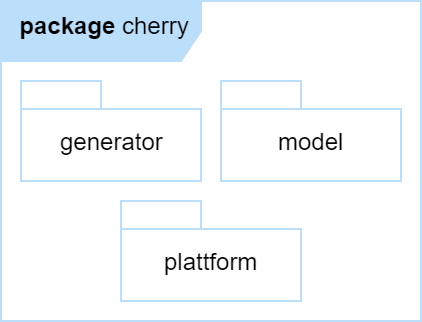
\includegraphics[width=0.5\textwidth]{bilder/cherry}
	\caption{Darstellung der Unter-Packages im cherry Package.}
	\label{fig:cherryPackages}
\end{figure}

\subsection{Cherry}

Aus den aus der Referenzimplementation entstandenen Annotations Modellen werden von Cherry im darauffolgenden Schritt die später verwendbaren Builder erzeugt. Zudem ist im Package model das von dieser generierten internen DSL beschriebene CodeUnit Modell definiert. Der im Konzept erwähnte Plattform Code ist in Cherry im Package platform zu finden. Abbildung~\ref{fig:cherryPackages} zeigt noch einmal die erwähnten Packages.

In den folgenden Abschnitten werden die Funktionsweise und Aufgabe von Cherry genau erläutert. Im Anschluss daran wird die Verwendung der erzeugten Bilder noch einmal erläutert und mit Beispiel verdeutlicht.

\subsubsection{CodeUnit Modell}

\begin{figure}[htbp]
	\centering
	\includegraphics[width=1.0\textwidth]{bilder/classCu}
	\caption{Klassen Diagramm des CodeUnit Modells.}
	\label{fig:classcu}
\end{figure}

Wie bereits zuvor erwähnt, könnte man das CodeUnit Modell als das Kernstück von Spectrum ansehen. Eine Instanz des CodeUnit Modells wird durch Verwendung der erzeugten internen DSL beschrieben und aus dieser kann dann zum Beispiel wieder konkreter Java Quelltext erzeugt werden.

Das Diagramm auf Abbildung~\ref{fig:classcu} zeigt das CodeUnitModell und seine Hilfsklassen.
Die Grundidee des CodeUnit Modells wurde im Konzeptkapitel bereits erläutert. Konkret wird der Zusammenhang zwischen CodeUnit und SubCodeUnits dadurch dargestellt, dass eine CodeUnit eine Liste mit weiteren CodeUnits hält. Der Typ der CodeUnit wird in einem Feld eines Wertes des CodeUnitType Enums gehalten. Es gibt nicht immer zwingend zu jedem CodeUnitType auch einen möglichen Builder. Die CodeUnitTypes METHOD\_BODY und METHOD\_PARAM existieren nur als SubCodeUnits des CodeUnitTypes METHOD.

Besonderes Augenmerk fällt hier darauf, dass in der Implementation, entgegen dem Konzept, von CodeUnit abgeleitete Klassen existieren. Wie bereits beschrieben, wird die Identifikation des Typs einer CodeUnit anhand des CodeUnitType durchgeführt. Die Ableitungen von CodeUnit haben keine eigene Funktion und dienen nur zur Fehlerreduzierung bei der Verwendung der Builder. Durch spezielle CodeUnit Klassen ist es möglich Builder Methoden zu generieren welche einschränken welche Art von CodeUnit als SubCodeUnit übergeben werden darf. Beispielsweise kann mithilfe der MethodCodeUnit Klasse eine Methode für ein Builder der eine ClassCodeUnit beschreibt erzeugt werden welche ausschließlich die Übergabe einer MethodCodeUnit erlaubt. Konkret wäre das die Methode withMethod.

Das Konzept der Parametrisierung durch eine generische Datenstruktur wurde als Map mit dem Schlüssel CodeUnitDatumType Einträgen des Typs CodeUnitDatum realisiert. CodeUnitDatumType ist abermals ein Enum welche später die semantische Information was der hinterlegte Parameter bedeutet. Der Parameter selbst, also das CodeUnitDatum, ist generisch Parametrisiert und kann somit einzelne Werte oder auch Arrays halten. Allgemein kann hier jedoch jeder Datentyp stehen, für den CodeUnitDatumType Identifier wird hier beispielsweise ein String als Typparameter verwendet. Zur Verdeutlichung zeigt Listing~\ref{lst:cud} die Implementation von CodeUnitDatum und exemplarisch wird in Listing~\ref{lst:cudex} dargestellt, wie einer CodeUnit ein CodeUnit Datum hinzugefügt werden kann und wie dieses später ausgelesen werden muss. 

Die Methode addCodeUnitDatum folgert den hinterlegten Datentyp anhand des als zweiten Parameter übergebenen Datums. Mit der Methode getCodeUnitDatum kann das unter einem CodeUnitDatumType hinterlegte Datum wieder ausgelesen werden. Da die Information welcher generische Typparameter in der Map hinterlegt wurde verloren geht, muss stets explizit auf den korrekten Typ umgewandelt werden. Dies stellte kein Problem dar, da unter einem bestimmten CodeUnitDatumType mit ein bestimmten Datentyp zu rechnen ist.

\begin{lstlisting}[label=lst:cud,
language=java,
firstnumber=1,
caption=Implementation der Klasse CodeUnitDatum.]
public class CodeUnitDatum<T> implements Serializable {
	private final T datumData;

	public CodeUnitDatum(T datumData) {
		this.datumData = datumData;
	}

	public T getDatumData() {
		return datumData;
	}

	@Override
	public String toString() {
	if(datumData.getClass().isArray())
		return Arrays.toString((Object[]) datumData);

	return datumData.toString();
	}
}
\end{lstlisting}

\begin{lstlisting}[label=lst:cudex,
language=java,
firstnumber=1,
caption=Beispiel zum konkreten hinterlegen und auslesen eines CodeUnitDatums.]
void exampleDatumWriter(String identifier) {
	CodeUnit cu = new CodeUnit();
	cu.addCodeUnitDatum(CodeUnitDatumType.IDENTIFIER, identifier);
}

String exampleDatumReader(CodeUnit cu) {
	return (String) cu.getCodeUnitDatum(CodeUnitDatumType.IDENTIFIER).getDatumData(); 
}
\end{lstlisting}

\subsubsection{DSL Generator}

Der BuilderGenerator folgt dem Konzept, dass jeder Builder Komponenten basiert ist. Die Komponenten hierbei sind die Builder Methoden. Zum einen sind diese durch die im Annotations Modell hinterlegten Variabilitäten vorgegeben und zum anderen aus dem Typ der von dem Builder beschriebenen CodeUnit ableitbar. Im Generator wird ein Builder dementsprechend auf Grundlage dieser Daten Stück für Stück zusammengebaut.

Im ersten Schritt wird die Referenzimplementation zu einer CompilationUnit geparsed. Diese wird dann von Amber verarbeitet, woraus eine Liste von Annotations Modellen entsteht. Aus jedem dieser Modelle wird dann ein Builder erzeugt. Der Klassenname des Builder setzt sich aus dem Identifier des Annotations Modells und dem Suffix UnitBuilder zusammen. Im Anschluss hieran werden, abhängig von der zu beschreibenden CodeUnit, aus einer Hilfsklasse, dem BuilderMethodTypeProvider, die Informationen abgefragt welche Standardmethoden der Builder benötigt. Mit der BuilderMethodFactory wird aus dieser BuilderMethodType Information eine entsprechender JavaPoet MethodSpec eurzeugt. Danach werden auf gleichem Weg die MethodSpecs zur Beschreibung der Variabilitäten erzeugt und angehängt.

Um die in der defaultCodeUnit hinterlegten Daten in die Ursprungs CodeUnit des Builders zu übertragen wird die Default CodeUnit zu einem Byte Array serialisiert. Dieses Byte Array wird als Literal in der erzeugten initializeDefaultCodeUnit Methode hinterlegt. Diese Methode wird im Konstruktor des erzeugten Builders aufgerufen und sorgt dafür das, dass aus dem Byte Array wieder ein CodeUnit Objekt deserialisiert wird. Die Erzeugung dieses MethodSpecs und die von JavaParser aus dem MethodSpec erzeugte Builder Methode werden in Listing~\ref{lst:defcu} gezeigt.

\begin{lstlisting}[label=lst:defcu,
language=java,
firstnumber=1,
caption=Quelltext zur Erzeugung des MethodSpecs für die Builder-Methode initializeDefaultCodeUnit und die daraus resultierende konrekte Methode in einem Builder.]

//Erzeugung des MethodSpec in der BuilderMethodFactory
private MethodSpec createInitDefCodeUnitMethod() {
	CodeUnit sourceCodeUnit = annotationModel.getDefaultCodeUnit();

	byte[] serializedCodeUnit = SerializationUtils.serialize(sourceCodeUnit);

	String codeUnitArrayLiteral = Arrays
		.toString(serializedCodeUnit)
		.replace("[","{")
		.replace("]","}");

	return MethodSpec.methodBuilder("initializeDefaultCodeUnit")
			.addComment("Initializes this builder's data with default data encoded into a byte[]")
			.addModifiers(Modifier.PRIVATE)
			.addStatement("byte[] serializedCodeUnit = new byte[] $L", codeUnitArrayLiteral)
			.addStatement("this.codeUnit = $T.deserialize(serializedCodeUnit)", SerializationUtils.class)
			.build();
}

//Erzeugte konrete Methode in einem Builder
private void initializeDefaultCodeUnit() {
	// Initializes this builder's data with default data encoded into a byte[]
	byte[] serializedCodeUnit = new byte[] {-84, -19, 0/* more data */};
	this.codeUnit = SerializationUtils.deserialize(serializedCodeUnit);
}
\end{lstlisting}

\subsubsection{Abhängigkeit der erzeugten Builder zu Plattform Code}

Um die erzeugte DSL verwenden zu können, muss das Package platform zur Verfügung stehen. Hierin befinden sich Klassen zur Auflösung von Referenzen und zur Fehlerbehandlung. Da Getter und Setter erst zur Laufzeit, während die Builder bereits im Einsatz sind, erzeugt werden können, findet sich hier auch der DefaultCodeUnitProvider. Im aktuellen Stand von Spectrum ist die Funktionalität der Plattform Klassen noch sehr beschränkt. Vor allem die Fehler Handhabung ist nur exemplarisch implementiert. Momentan werden nur Klassen Referenzen auf die beschriebene Klasse selbst aufgelöst, um für den Proof of Concept die Definition von Singletons mithilfe der internen DSL möglich zu machen. Da die Referenz auf Basis eines CodeUnitDatums aufgelöst wird, könnten selbst verständlich noch weitere Referenzen im Parse Prozess hinterlegt werden und somit auch vom CodeUnitReferenzResolver gehandhabt werden.

\subsubsection{Verwendung der erzeugten Builder}

Listing~\ref{lst:exb} stellt die Anwendung der generierten Builder dar. Anzumerken ist, dass dieses Beispiel eine kaum sinnhafte CodeUnit beschreibt und lediglich die verschiedenen Möglichkeiten und wie man die einzelnen Builder Methoden anwendet aufzeigt.

Modifier werden mit einem Enum gehandhabt. Methoden welche einen Datentypen als Parameter erwarten bekommen diesen als String übergeben. Ein einfacher Weg diesen zu erhalten ist über die Klasse mit .class auf die Methode getName zuzugreifen. Der Körper einer Methode wird hier, genau wie bei JavaPoet, als String übergeben.

Ein zusammenhängendes Beispiel wie aus einer Referenzimplementation mit Annotationen Builder generiert werden, wie man diese dann benutzen kann und wie daraus generierter Java Quelltext aussieht, folgt am Ende dieses Kapitels.

\begin{lstlisting}[label=lst:exb,
language=java,
firstnumber=1,
caption=Quelltext zur Verwendung verschiedener erzeugter Builder.]
CodeUnit cu = ExampleClassUnitBuilder
				.createWithIdentifier("ExampleIdentifier")
				.withModifiers(CodeUnitModifier.PROTECTED)
				.withField(VarUnitBuilder
					.createWithIdentifier("exampleField")
					.withModifiers(CodeUnitModifier.PRIVATE)
					.withDataType(Object.class.getName())
					.end())
				.withMethod(MethodUnitBuilder
					.createWithIdentifier("exampleMethod")
					.withModifiers(CodeUnitModifier.PUBLIC)
					.withParameter("param", String.class.getName())
					.withMethodBody("return param")
					.withReturnType(String.class.getName())
					.end())
				.withConstructor(ConstructorUnitBuilder
					.create()
					.withParameter("param", String.class.getName())
					.withModifiers(CodeUnitModifier.PUBLIC)
					.withMethodBody("//body als String")
					.end())
				.end();
\end{lstlisting}

\subsection{Jade}

Die eher kleine Komponente Jade hat zur Aufgabe fertig beschriebene CodeUnits in ein für Scarlet verarbeitetbares Modell zu transformieren. Jade umfasst nur das Package transformator, in welchem auch nur die Klasse CodeUnitTransformator liegt.

\subsubsection{Transformator}

Für die unterschiedlichen Elemente in Scarlet's Java Modell sind im CodeUnitTransformator Transformationsregeln in Form von Methoden definiert. Da das CodeUnitModell und somit auch die CodeUnitTypes ursprünglich aus Java Quelltext abgeleitet wurden, ist die Umwandlung vergleichsweise unkompliziert. Dies ist am Beispiel der Transformation von Feldern in Listing~\ref{lst:trans} gut zu sehen. Mithilfe von Java-Streams werden hier die SubCodeUnits einer Klassen CodeUnit gefiltert und dann die einzelnen Felder umgewandelt.

\begin{lstlisting}[label=lst:trans,
language=java,
firstnumber=1,
caption=Umwandlung der Felder in den SubCodeUnits einer CodeUnit. Auszug aus der Klasse CodeUnitTransformator.]
private List<JavaField> transformFields(CodeUnit cu) {
	return cu.getSubCodeUnits()
				.stream()
				.filter(this::isField)
				.map(this::transformField)
				.collect(Collectors.toList());
}

private JavaField transformField(CodeUnit cu) {
	JavaField jField = new JavaField();
	jField.modifiers = this.transformModifier(cu);
	jField.identifier = this.transformIdentifier(cu);
	jField.type = this.transformType(cu);
	jField.typeParams = this.transformTypeArguments(cu);
	
	return jField;
}
\end{lstlisting}

\subsection{Scarlet}

Die Komponente Scarlet stellt ein Modell zur Verfügung welches die Struktur und den Aufbau einer Java Klasse widerspiegelt. Die zweite Aufgabe von Scarlet ist es aus diesem Java Modell konkreten Java Quelltext zu erzeugen. Die in Scarlet definierten Visitor finden keine Verwendung mehr, ursprünglich haben diese Java Quelltext eingelesen und in das Java Modell überführt.

\subsubsection{Allgemeiner Java Klassen Generator}

Der Generator ist vergleichsweise einfach aufgebaut. Der konkrete Quelltext wird abermals mit Java Poet erzeugt. Für die unterschiedlichen im Java Modell darstellbaren Java Elemente sind in der Klasse JavaClassGenerator jeweils generate Methoden implementiert. Diese Methoden erzeugen die für JavaPoet notwendigen Objekte. Mithilfe des JavaPoetTypeMappers werden die als Zeichenketten vorliegenden Klassennamen zu einem JavaPoet Type umgewandelt.

\subsubsection{Modell zur Abbildung von Java Klassen}

Das Modell auf dessen Basis Scarlet den Java Quelltext erzeugt, ist ein Teilmodell des Java Metamodells. Soll Spectrum um neue generier Möglichkeiten erweitert werden, so werden auch meist das Scarlet Java Modell und der Java Klassengenerator ergänzt.

\subsection{Violet}

Als letzte und auch kleinste Komponente stellt Violet einen Logger zur Verfügung. Dies ermöglicht es vereinfacht eine Info- oder Fehlernachricht auf der Konsole auszugeben. Er sollte leicht um Ausgabe in einer Log-Datei erweiterbar sein.

\section{Erweiterung von Spectrum}

Im letzten Abschnitt dieses Kapitels wird beschrieben wie ein beispielhafter Erweiterungsprozess für Spectrum aussehen könnte. Hierdurch sollen Anhaltspunkte gegeben werden welche Komponenten und Klassen für eine Ausweitung des Funktionsumfangs bearbeitet werden müssen.

Allgemein gilt bei der Erweiterung von Spectrum immer das gleiche Prinzip. Soll eine neue Annotation hinzugefügt werden muss in Amber diese Annotation definiert werden und im Modell muss das Annotation Type Enum erweitert werden. In jedem Fall muss der entsprechende Annotation Parser die gewünschten neuen Daten aus dem AST in das Annotations Modell übertragen. 

Der einfachste Fall ist die Erweiterung der möglichen Ziele für FixedCodeUnit. Zuerst müssen die möglichen Targets der FixedCodeUnit entsprechend erweitert werden. Dies geschehen sollten ein neuer Visitor und ein neuer Parser für das neue Ziel erstellt werden, hierbei kann man sich gut an der vorhandenen Struktur orientieren. Intern sind die Parser sehr ähnlich aufgebaut, für die Annotation direkt und Annotationen die in Abhängigkeit der Haupt Annotation stehen, gibt es jeweils parse Methoden. Für die FixedCodeUnit wird eine parseFixedCodeUnitAnnotation Methode implementiert welche prüft ob die entsprechende Annotation vorhanden ist und wenn ja, die vorhandene defaultCodeUnit des Modells um die neuen FixedCodeUnit Daten erweitert. Bei Bedarf können neue CodeUnitTypes und CodeUnitDatumTypes angelegt werden. 

Da es sich hier um eine FixedCodeUnit handelt müssen keine neuen Builder Methoden erzeugt werden. Um später Java Quelltext erzeugen zu können muss zuerst das Java Modell von Scarlet um entsprechende Klassen oder Felder erweitert werden. Danach können im JavaClassGenerator neue generate Methoden implementiert werden. Der letzte Schritt ist dann in Jade neue Transformationsregeln zu definieren, welche die Daten der CodeUnit in Java Modell Daten umwandeln.

Bei der Entwicklung von Spectrum wurde die Erfahrung gemacht, dass eine Erweiterung fast jedes Mal ein Element sowohl als FixedCodeUnit Annotierbar sein soll, als auch als Variabilität von einem Builder beschreibbar. Da, wie oben beschrieben, bei einer FixedCodeUnit keine Erweiterung des BuilderGenerators notwendig ist, ist es sehr hilfreich zuerst den gesamten Erweiterungsprozess für eine FixedCodeUnit durchzuführen und sich dann erst um die Implementation der fehlenden Teile für die CodeUnit Annotation kümmert.

Handelt es sich um eine neue Variabilität die mit der internen DSL ausgedrückt werden können soll, muss zuerst die BuilderMethodFactory um die neue Methode erweitert werden. Parallel dazu wird ein neuer BuilderMethodType hinzugefügt. Jetzt kann dafür Sorge getragen werden dass Amber im entsprechenden Parser die für den Generator notwendige Information, dass eine entsprechende Methode generiert werden soll, als Variabilitäts Annotation aufnimmt. Wurden die oben erwähnten Schritte für die FixedCodeUnit bereits einmal implementiert, wäre die Erweiterung jetzt abgeschlossen.

Natürlich, vor allem Zusammenhang mit Erweiterungs Annotationen, können die einzelnen Schritte mehr oder weniger komplex ausfallen oder es könnten grundsätzliche Änderungen an Spectrum notwendig sein. Diese Fälle können in dieser Arbeit jedoch nicht alle abgehandelt werden, der diese kaum absehbar sind.

\section{Zusammenhängendes Beispiel: Von der Referenzimplementation zum erzeugten Java Quelltext}

\begin{lstlisting}[label=lst:java,
				   language=java,
				   firstnumber=1,
				   caption=Beispiel für einen Quelltext]

public void foo() {
	// Kommentar
}
\end{lstlisting}

\chapter{Evaluierung}
\section{Kozept \& Implementation}
\subsection{Amber}
\subsection{Cherry}
\subsection{Jade}
\subsection{Scarlet}
\section{Softwarequalität}
Nach Balzert S.111
\subsection{Functionality}
\subsection{Maintainability}
\subsection{Performance}
\subsection{Usability}
\section{Grenzen des Lösungsansatzes}

\chapter{Abschluss}
\section{Zusammenfassung}
\section{Ausblick}

\appendix
\chapter{Dokumentation}
\section{Verwendung der Annotationen}
\section{Verwendung der generierten CodeUnit-Builder}
\section{Klassendokumentation}
\subsection{Amber}
\subsection{Cherry}
\subsection{Jade}
\subsection{Scarlet}


\backmatter
%%%%%%%%%%%%%%%%%%%
%% create  list
%%%%%%%%%%%%%%%%%%%

\listoffigures
\addcontentsline{toc}{chapter}{Verzeichnisse}

%%%%%%%%%%%%%%%%%%%
%% create tables list
%%%%%%%%%%%%%%%%%%%
\listoftables

%%%%%%%%%%%%%%%%%%%
%% create listings list
%%%%%%%%%%%%%%%%%%%
%\lstlistoflistings
%\addcontentsline{toc}{chapter}{Listings}

\printbibliography
\addcontentsline{toc}{chapter}{Literatur}

%%%%%%%%%%%%%%%%%%%
%% declaration on oath
%%%%%%%%%%%%%%%%%%%

\addchap{Eidesstattliche Erklärung}

Hiermit versichere ich, dass ich die vorgelegte Bachelorarbeit selbstständig verfasst und noch nicht anderweitig zu Prüfungszwecken vorgelegt habe. Alle benutzten Quellen und Hilfsmittel sind angegeben, wörtliche und sinngemäße Zitate wurden als solche gekennzeichnet.

\vspace{20pt}
\begin{flushright}
$\overline{~~~~~~~~~~~~~~~~~\mbox{\BaAuthor, am \today}~~~~~~~~~~~~~~~~~}$
\end{flushright}

\addchap{Zustimmung zur Plagiatsüberprüfung}

Hiermit willige ich ein, dass zum Zwecke der Überprüfung auf Plagiate meine vorgelegte Arbeit in digitaler Form an PlagScan (www.plagscan.com) übermittelt und diese vorrübergehend (max. 5~Jahre) in der von PlagScan geführten Datenbank gespeichert wird sowie persönliche Daten, die Teil dieser Arbeit sind, dort hinterlegt werden.

\begin{small}
Die Einwilligung ist freiwillig. Ohne diese Einwilligung kann unter Entfernung aller persönlichen Angaben und Wahrung der urheberrechtlichen Vorgaben die Plagiatsüberprüfung nicht verhindert werden. Die Einwilligung zur Speicherung und Verwendung der persönlichen Daten kann jederzeit durch Erklärung gegenüber der Fakultät widerrufen werden.
\end{small}

\vspace{20pt}
\begin{flushright}
$\overline{~~~~~~~~~~~~~~~~~\mbox{\BaAuthor, am \today}~~~~~~~~~~~~~~~~~}$
\end{flushright}

\end{document}
